% vim:ts=4:sw=4
%
% Copyright (c) 2008-2009 solvethis
% Copyright (c) 2010-2015 Casper Ti. Vector
% Public domain.
%
% 使用前请先仔细阅读 pkuthss 和 biblatex-caspervector 的文档,
% 特别是其中的 FAQ 部分和用红色强调的部分。
% 两者可在终端/命令提示符中用
%   texdoc pkuthss
%   texdoc biblatex-caspervector
% 调出。

% 采用了自定义的(包括大小写不同于原文件的)字体文件名,
% 并改动 ctex.cfg 等配置文件的用户请自行加入 nofonts 选项;
% 其它用户不用加入 nofonts 选项,加入之后反而会产生错误。
\documentclass[UTF8]{pkuthss}

% 使用 biblatex 排版参考文献,并规定其格式(详见 biblatex-caspervector 的文档)。
% 这里按照英文文献在前,中文文献在后排序(“sorting = ecnty”);
% 若需按照中文文献在前,英文文献在后排序,请设置“sorting = centy”;
% 若需按照引用顺序排序,请设置“sorting = none”。
\usepackage[backend = biber, style = caspervector, utf8, sorting = none]{biblatex}
%\usepackage[caption=false,font=footnotesize]{subfig}
\usepackage{multirow}
\usepackage{ntheorem}

\graphicspath{{../figure/}}
\DeclareGraphicsExtensions{.eps,.pdf, .jpg}

% 按学校要求设定参考文献列表中的条目之内及之间的距离。
\setlength{\bibitemsep}{3bp}
% 对于 linespread 值的计算过程有兴趣的同学可以参考 pkuthss.cls。
\renewcommand*{\bibfont}{\zihao{5}\linespread{1.27}\selectfont}

% 设定文档的基本信息。
\pkuthssinfo{
	cthesisname = {硕士研究生学位论文}, ethesisname = {Master Thesis},
	ctitle = {物理不可克隆函数的建模与~~设计研究},
	etitle = {Modeling and Design of Physical Unclonable Functions},
	cauthor = {唐~文~懿},
	eauthor = {Wenyi Tang},
	studentid = {1301214150},
	date = {二〇一六 年 四 月},
	school = {信息科学技术学院},
	cmajor = {微电子学与固体电子学}, emajor = {Microelectronics},
	direction = {系统集成芯片设计及设计方法学},
	cmentor = {贾嵩~~副教授}, ementor = {Prof.\ Song Jia},
	ckeywords = {物理不可克隆函数,建模攻击,FPGA,密码学},
	ekeywords = {Physical Unclonable Function, Modeling attack, FPGAS, Cryptography}
}
% 载入参考文献数据库(注意不要省略“.bib”)。
\addbibresource{thesis.bib}

\begin{document}
	% 以下为正文之前的部分,默认不进行章节编号。
	\frontmatter
	% 此后到下一 \pagestyle 命令之前不排版页眉或页脚。
	\pagestyle{empty}
	% 自动生成封面。
	\maketitle

	% 此后到下一 \pagestyle 命令之前正常排版页眉和页脚。
	% 封面要求单面打印,故需新开右页,此处已一并实现。
	\cleardoublepage
    \pagestyle{plain}
	% 重置页码计数器,用大写罗马数字排版此部分页码。
	\setcounter{page}{0}
	\pagenumbering{Roman}
    
	% 版权声明。
	% % vim:ts=4:sw=4
%
% Copyright (c) 2008-2009 solvethis
% Copyright (c) 2010-2015 Casper Ti. Vector
% All rights reserved.
%
% Redistribution and use in source and binary forms, with or without
% modification, are permitted provided that the following conditions are
% met:
%
% * Redistributions of source code must retain the above copyright notice,
%   this list of conditions and the following disclaimer.
% * Redistributions in binary form must reproduce the above copyright
%   notice, this list of conditions and the following disclaimer in the
%   documentation and/or other materials provided with the distribution.
% * Neither the name of Peking University nor the names of its contributors
%   may be used to endorse or promote products derived from this software
%   without specific prior written permission.
%
% THIS SOFTWARE IS PROVIDED BY THE COPYRIGHT HOLDERS AND CONTRIBUTORS "AS
% IS" AND ANY EXPRESS OR IMPLIED WARRANTIES, INCLUDING, BUT NOT LIMITED TO,
% THE IMPLIED WARRANTIES OF MERCHANTABILITY AND FITNESS FOR A PARTICULAR
% PURPOSE ARE DISCLAIMED. IN NO EVENT SHALL THE COPYRIGHT HOLDER OR
% CONTRIBUTORS BE LIABLE FOR ANY DIRECT, INDIRECT, INCIDENTAL, SPECIAL,
% EXEMPLARY, OR CONSEQUENTIAL DAMAGES (INCLUDING, BUT NOT LIMITED TO,
% PROCUREMENT OF SUBSTITUTE GOODS OR SERVICES; LOSS OF USE, DATA, OR
% PROFITS; OR BUSINESS INTERRUPTION) HOWEVER CAUSED AND ON ANY THEORY OF
% LIABILITY, WHETHER IN CONTRACT, STRICT LIABILITY, OR TORT (INCLUDING
% NEGLIGENCE OR OTHERWISE) ARISING IN ANY WAY OUT OF THE USE OF THIS
% SOFTWARE, EVEN IF ADVISED OF THE POSSIBILITY OF SUCH DAMAGE.

\specialchap{版权声明}

任何收存和保管本论文各种版本的单位和个人,
未经本论文作者同意,不得将本论文转借他人,
亦不得随意复制、抄录、拍照或以任何方式传播。
否则一旦引起有碍作者著作权之问题,将可能承担法律责任。

% 若需排版二维码,请将二维码图片重命名为“barcode”,
% 转为合适的图片格式,并放在当前目录下,然后去掉下面 3 行的注释。
%\vfill\noindent
%\includegraphics[height = 5em]{barcode}


    
	% 中英文摘要。
	% vim:ts=4:sw=4
% Copyright (c) 2014 Casper Ti. Vector
% Public domain.

\begin{cabstract}
信息安全是现在各项系统设计重中之重,单向函数是信息安全协议的基础之一。物理不可克隆函数(PUF)是实现单向函数的一种物理手段,利用未知物理系统的观测点实现激励到响应的映射函数。
PUF适合于有安全性需求的移动端芯片,有着低功耗、高集成度、高安全性等特点。

本文研究了 PUF 在电路系统的实现方法,论文的主要工作和创新点包括:
第一,利用统计方法对现有的多种 PUF 方案进行分析对比,建立数学模型描述电路行为,并从模型特征总结出各 PUF 优劣。
第二,提出了延迟型双稳态 PUF 设计方案,其结合了仲裁型 PUF 和双稳态 PUF 的优点,改进了双稳态 PUF 响应存在偏置的不足,且在 FPGA 上实现了电路并采样验证。
第三,设计了随机脉冲采样 PUF,该结构利用短脉冲传播的不稳定特性,引入随机变量,使得电路行为更加难以建模预测,增强了其抵御建模攻击的能力;同时通过真负边沿采样异或运算,增加了建模的空间复杂度,使得攻击者需要极大量的运算代价对此结构进行建模。最终实验结果显示,设计二具有极好的统计结果和抗建模攻击的能力,其面积开销也是标准 2-XOR PUF 的一半。

最后本文比较了新提出结构在内的多个 PUF 的统计分布、 NIST 测试结果和 SVM 预测结果。
	
\end{cabstract}

\begin{eabstract}
Modern system design concerns more and more about security. As one of the basic foundation of crypto-protocols, one-way function and its implementation takes efforts to do so. Physical Unclonable Functions (PUF) is an alternative to one-way function. PUF ultilizes physical system which is unknown to mankind to set up a projection from challenges to responses. This physical disorder based system, which has low energy consumption and high density, is quite suitable for security portable chips.

In this paper, we analyze and implment PUF in Field Programmable Gate Array, and investigate the randomness, uniqueness and reliability of the PUFs.
We also build models for these PUFs and extract characteristics from the model.
We propose two novel PUF designs. One of them combines the advantage of arbiter PUF and bistable ring PUF, the experiments on FPGA demonstrate it improves the randomness and uniqueness compared to BRPUF.
The other one refered to as random pulse based arbiter PUF, introduces a random bit with a random input pulse signal to confuse the one who wants to model it. The experiment results show the propsoed RPAPUF has a significant increment on space and time complexity of building a model for it.

In the end, we summarize the NIST test results and SVM learning results for all mentioned PUFs.

\end{eabstract}


	% 自动生成目录。
	\tableofcontents

	% 以下为正文部分,默认要进行章节编号。
	\mainmatter
	% 序言。
	% vim:ts=4:sw=4
% Copyright (c) 2014 Casper Ti. Vector
% Public domain.

\specialchap{序言}
信息安全是人类关注的永恒话题。而现代信息安全的大厦是由各种密码协议砌成的,这座大厦的基础就是构筑协议的数学原理。

古典密码学采用的简单映射,如凯撒密码,仿射密码,将原文字符通过线性变换映射成密文字符。由于线性变换的对称性,使得求解逆函数非常容易,这让简单映射密码非常容易受到攻击。最早的非线性加密手段——一次一密密码本——通过不断更换密码表(一种简单哈希表)达到非线性化的目的,只要密码本换的足够勤,那理论上就是不可破解的算法。

现代密码学运用了更深刻的数学知识。以对称加密算法 AES 为例, 128bit AES 加密需要10轮,每一轮都要经过一个非线性运算——S盒——求多项式在$GF(2^n)$上的逆。求逆之后,密钥的每一位都会与明文发生作用,这便使得逆向求解(已知密文、明文求解密钥)非常困难。又来看经典公钥算法 RSA,其用两个大质数分别作为公钥和私钥,利用一种单向函数``大整数的因式分解''使正向运算(求大质数的乘积)简单,而逆向运算(求大整数的因数)非常困难来保证安全性。由此可见,单向函数( One-Way Function )是密码学的基础之一。1945年克劳德·香农( Claude E Shannon )在其经典著作《密码学的数学原理》\supercite{shannon1945mathematical} 指出密码设计的两个原则:扩散( Diffusion )和扰乱( Confusion ),这两个原则也是构造单向函数的原则。扩散指输入变化 1bit 会使输出变化 50\% 的 bits,扰乱指输出的每一个 bit 都是由尽可能多的输出 bit 决定。

在众多的密码系统中,单向函数往往由纯数学概念构造,比如大整数因式分解( RSA )、椭圆曲线求解( ECC )、矩阵分解\supercite{wendt2013bidirectional}( DBF )等等,在实际的电路实现上往往硬件规模较大,或是求值时间较长,在现今有越来越多的便携设备接入网络,而在公共场合下有加密通信的需求,传统的加密方式便不适合应用在这些设备上,所以需要低功耗、低硬件开销的加密方案。

其次,各种便携设备不同于传统主机,流动性大,使得其本身容易被攻击者获取(比如丢失、遭克隆等等手段,而传统攻击者获取的仅仅是信道信息),这使得以物理手段获取旁道信息破译的方法在近几年尤为引人关注。旁道信息是与密文相关的中间信息,呈现方式有很多种,比如加密操作时的功耗、电磁辐射、热辐射、运算错误、存储介质状态等等。利用这些信息,可以快速的破译一些加密系统。如差分功耗分析法,通过相似操作的功耗差值来判断猜解密钥的正确性,大幅度削减了穷举量;又如错误分析,通过手段注入使加密系统产生运算错误,并根据出现错误的时机和现象筛选密钥;而存储介质的分析则通过电磁探测等手段直接观察存储器中的逻辑值,从而提取出关键信息。

针对每一种不同的攻击手段,必须分别采取防御措施。如针对差分功耗分析,使用随机掩码隐藏真正的功耗信息,增加攻击者破解的成本;针对错误注入,加入探测机制阻止系统在出错的时候暴露关键信息;而针对存储介质的攻击,则可以采用 PUF 技术隐式存储关键数据。

在 PUF 技术出现之前,双方通信中关键的密钥往往直接存储在非易失性存储器(如只读存储器 ROM )中。比如门禁系统中门卡的 RFID,只能保存在门卡自身的芯片内。尽管通信协议可以很好的加密通信信道内的数据,但是却不能保护芯片内部 ROM 中的信息。一个恶意攻击者一旦获取了一个门卡,则可以通过技术手段探查 ROM 中的数据提取出关键信息。而 PUF 则以加密系统的物理实现自身特点存储信息,相较于 ROM 等传统非易失性存储器,具有隐秘性好,不可探查等特点,因此受到了相关领域研究者的广泛关注。


Physical Unclonable Function( PUF )最早由 MIT 的理学博士 Pappu S. Ravikanth 于 2001 年提出\supercite{pappu2002physical},而其最初被称为 Physical One-Way Function 。 Ravikanth 在论文中提出了利用可测系统的未知物理状态构造一种 Hash 函数,函数的映射方式由系统的物理特性决定。这种系统必须具有可观测的量以提供输出,同时以人类现有的知识或计算能力不能仿真或计算系统内部的细节,这样攻击者便不会知道系统将提供什么样的输出。 Ravikanth 最后用光学系统实现了他的构想。 PUF 一词则由同是 MIT 的 B. Gassend 等人提出\supercite{gassend2002silicon},值得一提的是, Gassend 将 PUF 的全称写作 Physical Random Function,并称为了不和``伪随机函数''( Pseudo-Random Function )混淆,而写作 Physical Unclonable Function,记作``PUF''。 Gassend 真正提出了基于硅基电路实现的 PUF,他用一系列双口交换器级联的方式,通过检测输出端口延迟先后,将工艺随机波动转换成电平逻辑输出,他的这种电路随后被称为 Arbiter-PUF。不仅如此, Gassend 还提出了一整套 PUF 系统的完善措施,包括输入、输出矫正和 PUF 的实际应用可能,并给出了基于 FPGA 的实验结果,可以说给后来的研究者奠定了完善的基础和研究模板。

自硅基 PUF 提出后, PUF 的研究逐渐演化为几个方向。其一是 PUF 安全性的研究,通过理论和实验提取 PUF 模型参数;其二是 PUF 电路结构的研究,追求更高的可靠性,低功耗和高集成度;其三是 PUF 的应用领域,构建基于 PUF 的密码协议。

2004 年 MIT 的 Daihyun Lim 在其硕士毕业论文\supercite{lim2005extracting}提出对 Arbiter-PUF 建模,并用支持向量机( SVM )拟合出 Arbiter-PUF 的模型参数,开启了机器学习对 PUF 的建模攻击领域。此后,接着机器学习崛起的东风, PUF 研究在攻防两方的博弈中迅速崛起,近几年来吸引了越来越多的研究者和相关会议关注这一领域。

到目前为止, PUF 技术尚未成熟到商用地步,主要有以下几个技术难点。
\begin{itemize}
\item 其一,需要稳定的生成关键数据。系统的物理特征易受环境变化、使用寿命等因素的影响,基于物理特征生成的数据必须克服物理特征波动带来的影响;
\item 其二,安全性。提取的物理特征应不易于被现有技术模拟,不能预测物理特征以破解出关键数据;
\item 其三,实用性。结合上两点,还必须易于实现,以现有技术能在较低成本下制作出来。
\item 最后, PUF 并不适合放在现有的安全系统中,因此有越来越多的文献着手搭建以 PUF 为核心的安全协议,相信随着 PUF 研究的不断深入以及成熟的安全协议的提出, PUF 将会成为安全领域的一颗新星。
\end{itemize}

本文在前人研究基础上,从基本原理入手,分析 PUF 的建模于仿真,针对机器学习建模攻击的应用和防范,主要研究成果有以下几点:
\begin{itemize}
\item 第一,理论分析。对已提出的 PUF 结构进行建模,通过该模型仿真分析其性能指标,成功通过机器学习拟合模型参数;
\item 第二,电路结构。改进 PUF 结构,设计新型的电路结构以达到较高安全性,尤其是对建模攻击的防范;
\item 第三,仿真与实验。在 FPGA 上实现改进电路,通过 PCI-E 接口与 PC 通信,收集并测试大量的输出数据验证其性能指标。
\end{itemize}

文章分为5个章节,此为序章。第\ref{chap:preliminary}章主要阐述本文设计的基础知识;第\ref{chap:buildingmodel}章说明建模方法和安全性理论证明;第\ref{chap:dbrpuf}、\ref{chap:rpapuf}章则阐述本文提出的两种改进结构以及在 FPGA 的实现方法和实验结果;最后第\ref{chap:conclusion}章进行总结和提出展望。

	% 各章节。
	% vim:ts=4:sw=4
% Copyright (c) 2014 Casper Ti. Vector
% Public domain.

\chapter{预备知识}\label{chap:preliminary}
% 中文测试文字。
本章将文中所需要涉及的必要知识进行梳理和阐述,相关概念的定义和简介,不涉及具体证明过程。

\section{PUF工作原理}%
\subsection{工艺涨落}%
集成电路芯片制作可分为设计——流片——验证三大环节。
其中设计者输出给流片厂商的是版图信息。版图则对应着制程中每一层掩膜版的图形,具体到晶体管设计上,版图包括了晶体管宽长比,掺杂区域,互联方式等信息,结合工艺常数,决定了晶体管的设计属性。
在实际流片中,图形转移过程存在套刻精度、刻蚀精度,以及掺杂过程中的退火控制精度等问题。这些操作在实际中存在不可避免的随机误差和系统误差。系统误差在晶圆片上表现为 TT, FF, SS, SF 等不同片区,而随机误差则使得每一颗芯片的时序特征不同,也就是每一个晶体管的表征阈值电压均不相同。
从根本上来说,由于测量系统的局限性,永远不可能复制原子的所有信息,也即不可能使制作后晶体管数值与设计值完全相同。故而误差的累积则造成了工艺涨落,即流片后的晶体管属性与设计属性存在偏差,且在统计学上偏差满足一定的分布规律,下一节将详细说明如何利用由工艺涨落带来的不匹配。
\subsection{信息转换}
由于无法控制工艺涨落的具体数值,也无法预测涨落的大小,因此``芯片制作''这个物理过程符合PUF所要求的``可测不可知''的物理系统,接下来阐述如何给出工艺涨落的观测点。

\begin{figure}[htb!]
\centering
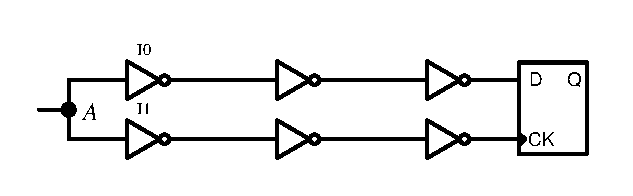
\includegraphics[width=.8\linewidth]{delay-puf}
\caption{延迟-仲裁型 PUF}
\label{fig:delay-puf}
\end{figure}
 
 \begin{figure}[htb!]
 \centering
 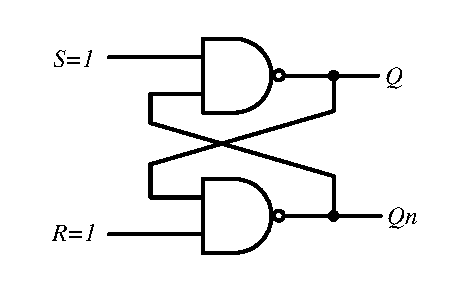
\includegraphics[width=.5\linewidth]{latch-puf}
 \caption{锁存式 PUF}
 \label{fig:latch-puf}
 \end{figure}

PUF将电路工艺参数涨落转换为可输出的电压或电流信号。如图\ref{fig:delay-puf}所示,其中每个反相器和相邻反相器之间的布线在设计上是全等的,但工艺涨落使得反相器中晶体管导电能力必有差异,那么反相器 $ I_0 $ 的信号延迟 $ \Delta t_0 $ 和 $ I_1 $ 的信号延迟 $ \Delta t_1 $ 定满足关系 $ \Delta t_0-\Delta t_1\neq 0 $ ,当输入一个上升沿信号 $ u(t) $ 后, A-D, A-CK  的延迟分别是 $ T_0,T_1 $ ,仲裁器负责判断 D 节点和 CK 节点信号跳变的先后,一个典型的D触发器即可满足仲裁功能。若 D 点信号先于 CK 点上跳,则仲裁器输出逻辑``1'',反之则输出逻辑``0''。由于在得到输出之前并不知道每个反相器的实际延迟,所以不能预测仲裁器的输出,而且每一块相同设计芯片之间的输出也因涨落分布的不同而有差异,因此这样的电路逻辑完成了从工艺涨落到电平信号的信息转换。

又如图\ref{fig:latch-puf}所示,两个反相器及布线在设计上是全等的,上电初始电路处于亚稳态,由于实际的反相器存在偏差,导致其中一个节点的充电电流稍大于另一个节点,使得电路大概率由亚稳态向其中一个稳态过度,此大概率得到的稳态也是工艺涨落的体现,这样的电路也完成了从工艺涨落到存储逻辑值的信息转换。值得注意的是,这里使用了``大概率''的说法,是因为在由亚稳态到稳态的弛豫时间中,存在噪声干扰,从而导致电路向工艺无关的方向变化,这是 PUF 设计中不愿看到的事情。有关 PUF 稳定性的问题,参见\ref{subsec:metrics}节。

\subsection{Weak PUF和Strong PUF}\label{subsec:weakpuf}
类似于\ref{fig:delay-puf}和图\ref{fig:latch-puf}中的电路,利用物理过程的不可控和不可预测性,表达一位或多位稳定信号的系统被称为物理不可克隆函数( Physically Unclonable Function ),其不一定局限于硅基电路,事实上, PUF 概念的首次提出是在光学系统上实现的\supercite{pappu2002physical}。

如果将图\ref{fig:latch-puf}中的结构排成阵列,加上行列选择和译码电路,则构成了类似 SRAM 的阵列,通过不同的``地址''信号可以输出不同的单元信息,像这样的``地址信号''在 PUF 中被称为激励( Challenge ),输出信号被称为响应( Response )。每一个响应都由一个激励相对应,将它们合称为激励-响应对( C-R Pair, CRP )。

\textbf{定义:}若一个 PUF 的激励响应对很少,则称其为 Weak PUF;反之,激励响应对数量级非常多的则称为 Strong PUF\supercite{ruhrmair2014pufs}。

Weak PUF CRP比较单一,没有对外的 IO 接口,以防被穷举,直接将生成的信号送入后续逻辑,实现方式有 SRAM PUF, SA PUF, Latch PUF 等等\supercite{schrijen2012comparative,koeberl2012practical,xiao2014bit,maes2014countering,bhargava2013high}, Weak PUF 多应用于随机数生成、密钥存储方面;

Strong PUF CRP空间非常大,存在对外的 IO 接口,允许通过输入不同的激励得到一组响应,而 CRP 集合的元素量级决定了不可能穷举完所有的 CRP。实现方式有 Arbiter PUF, RO PUF 等等,可实现多种协议。

可以看出 Weak PUF 和 Strong PUF 只是人为地划分,没有明确界限,相较而言,目前以 Strong PUF 的研究和应用居多\supercite{rostami2014quo}。

\subsection{评价指标}\label{subsec:metrics}
PUF (这里特指 Strong PUF,后同)可以用以下几个特定指标衡量:
\begin{itemize}
\item 随机性——对任何一个 CRP 集合的子集,响应(简称 R,后略)的分布应尽可能满足平均分布;
\item 独特性——对任何一个特定的激励(简称 C,后略),一组 PUF 的响应的分布应尽可能满足平均分布;
\item 可靠性——对同样的激励在不同环境温度、电源电压下重复操作应给出相同或大概率相同的响应;
\item 安全性——应对各种已知攻击,详见下一节。
\end{itemize}

除此之外,还有电路通用的面积、功耗、速度等指标,也有用NIST,熵等统计工具代替上述公式\supercite{van2013bias,koeberl2014entropy},特定指标优先级高于通用指标。

下面给出1-3指标的数学定义:

设激励 C 集合$ {c_i} $,响应 R 集合$ {r_i} $,$ r_i=f(c_i) $,若$ R={0,1} $,则随机性可以表征为:
\begin{equation}\label{eq:metric-rand}
Rand=\frac{1}{N}\cdot\sum^{N}f(c_i)
\end{equation}
$ N $ 为 CRP 测试集元素总数,随机性期望值为$ 0.5 $,表明响应应在随机选取的激励下呈平均分布;

独特性表征为:
\begin{equation}\label{eq:metric-uniq}
Uniq=\dfrac{2}{M(M-1)}\sum_{i=1}^{M}\sum_{j=i+1}^{M}\frac{HD(P_i,P_j)}{N}
\end{equation}
\begin{equation}\label{eq:metric-uniq2}
P_i=<f_i(c_0),f_i(c_1),...,f_i(c_n)>
\end{equation}
其中 $ M $ 为测试 PUF 设备总数, $ N $ 为测试激励总数, $ P_i $ 为第 i 个设备 N 个激励响应组成的向量, $ HD(P_i,P_j) $ 指 $ P_i,P_j $ 之间的汉明距离。
独特性期望值为$ 0.5 $,表明任意激励的响应在不同设备间应呈平均分布;

可靠性表征为:
\begin{equation}\label{eq:reliability}
Reliability=\dfrac{1}{MN}\sum_{j}^{M}\sum_{i}^{N}|f(c')-f^{(j)}(c_i)|
\end{equation}
其中N为测试激励总数, $ M $ 为测试重复次数, $ c’ $ 为参考激励,保持不变。可靠性期望值为0。


\section{PUF安全性问题}\label{sec:puf_security}

\subsection{物理模型}
虽然不能精确模拟流片时的掺杂、退火等行为,但是还是可以从宏观上表征一个 PUF 的行为,成这种方式为建模。通常可以将门级电路的驱动能力、延时等抽象为一个平均值W,将R视为C和W的映射 $ R=f(C,W) $。同时,一个好的物理模型有助于快速且准确的仿真验证。

\subsection{参数拟合}
由于 Strong PUF 开放IO端口的特点,若根据攻击者已掌握的一组 CRP 子集,根据建模特点,用机器学习算法拟合出抽象参数$ W $,便可将$ C,W $带入模型中得到 CRP 全集,根据预测率的高低可确定模型建立是否准确抽象了 PUF 的特点。严格来讲,如果一类 PUF 可以被准确抽象出模型,则称该 PUF 是不安全的。但考虑到不是所有模型都能在有限时间内拟合出参数,所以一般认为在特定场合可接受的时间内不能被拟合出参数的 PUF 是安全的。

\section{机器学习算法简介}

\subsection{支持向量机}
支持向量机(Support Vector Machine,SVM),是一种经典的模式识别算法,是 Bell 实验室的 Corinna Cortes 和 Vladimir Vapnik 于1995年首先提出的算法,后经改进,广泛应用于非线性函数拟合,模式识别等机器学习应用中\supercite{cortes1995support}。

SVM 的基本思想是将输入数据映射到一个n维空间中,找到n维空间中的一个超平面能将测试数据集划分开,则该平面将整个空间划分为二,对应着两类不同的数据(如图所示)。

\begin{figure}[h]
\centering
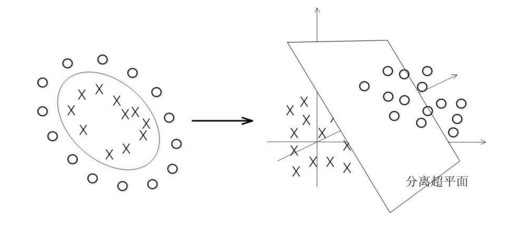
\includegraphics[width=\linewidth]{svm_teach.jpg}
\caption{SVM 映射示意图}
\label{fig:svm_proj}
\end{figure}

下面我们给出线性 SVM 的描述。考虑在n维空间中存在m个特征向量 $ x_1,x_2,x_3,…,x_m $,每个向量具有一个标签( label )``0''或者``1'',期望找到一个超平面( Hyperplane )
\begin{equation}
g(x)=w'x+b=0
\end{equation}
其中 $ w $ 和 $ b $ 是超平面的系数向量。$ g(x) $可以将特征向量分为两类,使得标签``1''向量都满足 $ g(x_i )>0 $,而标签``0''向量都满足 $ g(x_i )<0 $。定义:
\begin{equation}
\gamma=\frac{g(x)}{||w||}
\end{equation}
为向量x到超平面$ g(x)=0 $的几何距离,其中
$ ||w||=\sqrt{w_1^2+w_2^2+...+w_n^2} $
是系数向量w的范数。
为了增加分类的可信度,我们需要找到一个超平面,使得所有特征向量到该超平面的几何距离最大。

事实上并不是所有的数据都是线性可分的,即不存在一个超平面可以将数据集按标签分开。因此非线性 SVM 的做法通常是:
将数据由n维空间映射到$ n+k $维,使得在$ n+k $为空间中数据线性可分。

\subsection{SVM与PUF建模攻击}
如果 PUF 的模型是 $ r=f(c)=sgn(\omega'c+b) $ 的形式,其中 r 是响应,c 是激励,$ \omega $ 是 PUF 内在属性,$ sgn() $是一个符号函数。可以看出 $ g(c)=\omega'c+b=0 $ 便类似于 SVM 中的超平面,在 c 所在空间中,$ g(c) $将向量 c 按标签 r 分为了两类。通过 SVM 找到使 $ \gamma=\frac{g(c)}{||\omega||} $最大的$ \omega $,以使模型达到最大可信度。 SVM 的求解过程在 Matlab 中以 SMO 算法封装实现,而且求解过程并不是本文的关注点,所以不在这里赘述。


\section{相关工作}\label{sec:relatedwork}
\subsection{仲裁型PUF}\label{subsec:apufmodel}
图\ref{fig:delay-puf}展示了一个简单的仲裁型 PUF,图\ref{fig:arb-puf}是一个完整的仲裁型 PUF。其中激励 $ c_i $ 控制双口交换器使得:
\begin{eqnarray}
O_0=c_i?I_1:I_0\\
O_1=c_i?I_0:I_1
\end{eqnarray}
$ O_0,O_1 $ 是交换器的输出, $ I_0,I_1 $ 是输入。这样不同的激励选定了不同的两条数据通路做延迟对比,使得 CRP 空间有 $ 2^n $ 个元素,n为级数。

\begin{figure}[htb!]
\centering
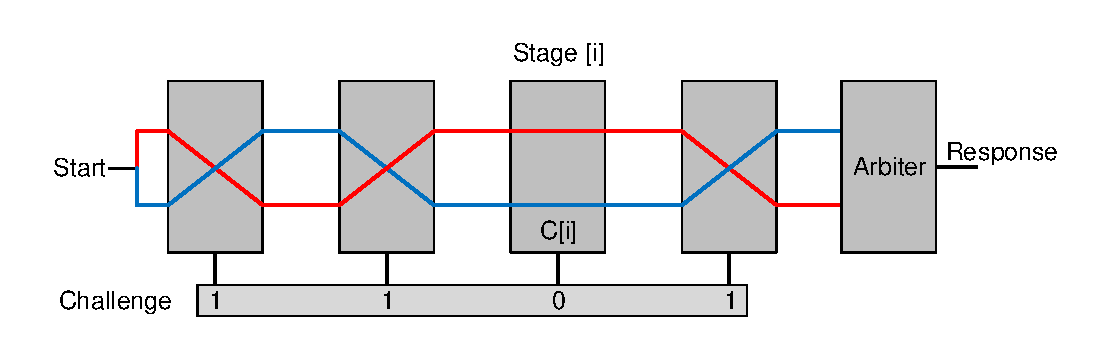
\includegraphics[width=\linewidth]{arbiter_puf}
\caption{仲裁型PUF}
\label{fig:arb-puf}
\end{figure}

将每一个交换器抽象为4条通路,设每条通路延迟分别为 $ p_i,q_i,r_i,s_i $ (如图\ref{fig: switcher}所示),信号到达输入的时间分别为 $ t_1(i),t_2(i) $,输出的时间分别为 $ t_1(i+1),t_2(i+1) $,则有:
\begin{eqnarray}\label{eq:apuf-cell}
t_1(i+1)=c_i?t_2(i)+r_i:t_1(i)+p_i \\
t_2(i+1)=c_i?t_1(i)+q_i:t_2(i)+s_i
\end{eqnarray}

\begin{figure}[htb!]
\centering
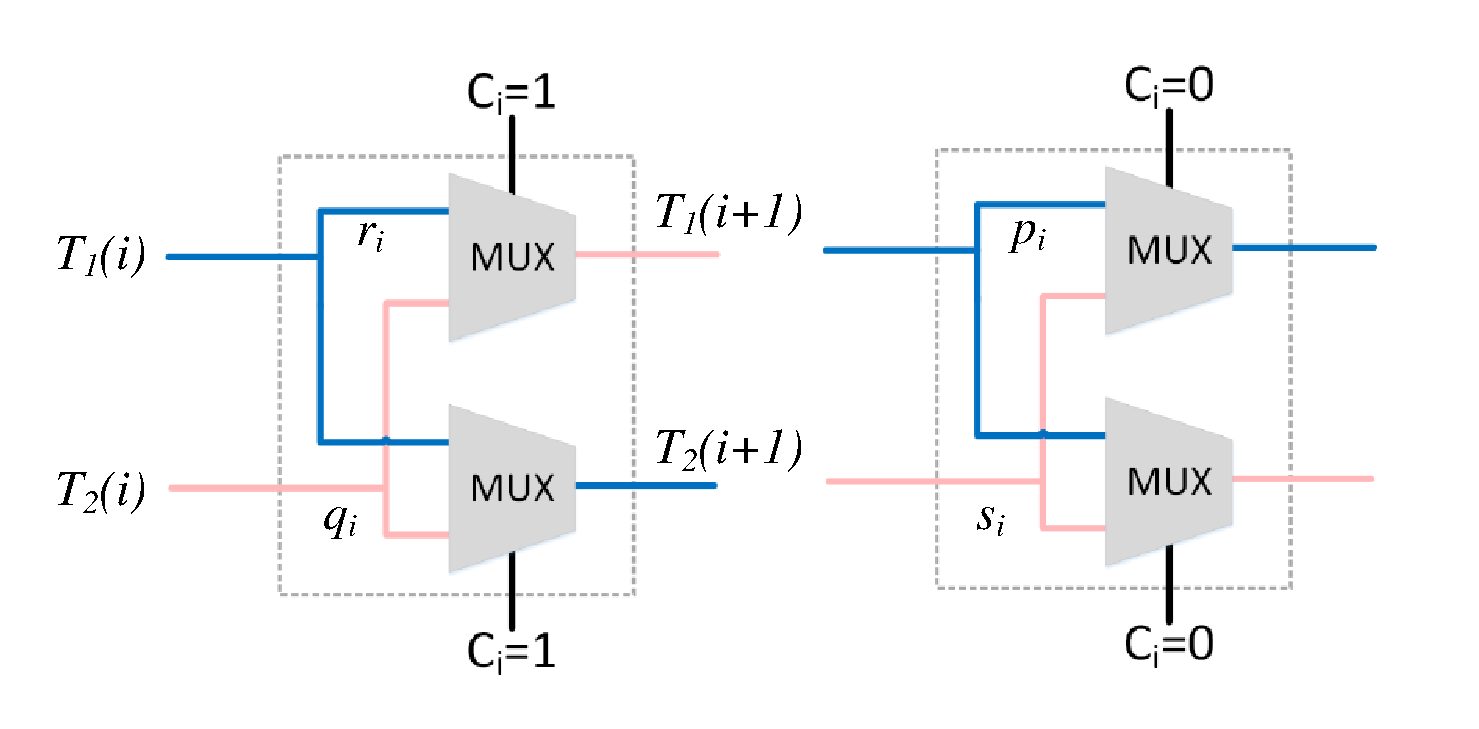
\includegraphics[width=\linewidth]{switcher}
\caption{双口交换器模型}
\label{fig: switcher}
\end{figure}

为了方便数学推导,将逻辑``0''记为-1,将逻辑``1''记为+1,则``异或''等价``乘''运算,故\ref{eq:apuf-cell}可化为
\begin{eqnarray}
t_1(i+1)=\frac{1+c_i}{2}(t_2(i)+r_i)+\frac{1-c_i}{2}(t_1(i)+p_i) \\
t_2(i+1)=\frac{1+c_i}{2}(t_1(i)+q_i)+\frac{1-c_i}{2}(t_2(i)+s_i)
\end{eqnarray}
两式做差得:
\begin{equation}
\delta (i+1)=t_1(i+1)-t_2(i+1)=-c_i\delta(i)+\frac{r_i-q_i+p_i-s_i}{2}+\frac{c_1}{2}(r_i-q_i-p_i+s_i)
\end{equation}
求解此递推关系式最终可得:
\begin{equation}
\delta(n)=p'd
\end{equation}
其中向量 $ p=<p_0,p_1,…,p_n> $, $ p_i=\Pi_{k=i+1}^{n}c_k $,向量 $ d=<\alpha_1,\alpha_2+\beta_1,…,\alpha_n+\beta_(n-1),\beta_n> $, $ \alpha_i=\frac{r_i-q_i-p_i+s_i}{2},\beta_i=\frac{r_i-q_i+p_i-s_i}{2} $,并定义 $ p_n $ 为常数1。由于 $ r=f(c)=sgn[\delta(n)] $,所以存在n维空间上的超平面 $ p'd=0 $ 将特征向量p按r标签分开。在这里p是向量c在同维空间中的一个映射,而向量d代表了每个交换器的延迟时间,是 PUF 的本征属性。

通过一组已知的 CRP 子集,我们可以确定一组向量d,用 SVM 算法找到具有最大可信度的d向量,作为延迟时间的估值,这样便推导出了仲裁型 PUF 的模型,对于未知响应的激励 $ c’ $,根据 $ sgn(p'd) $ 可预测其响应。根据文献\parencite{lim2005extracting}的数据,当训练集大小超过2000时,预测准确率在95\%以上。

\subsection{仲裁型PUF的改进}
因为仲裁型 PUF 的观测点——延迟时间的累加是线性过程,所以容易建立适合 SVM 算法的模型。在文献\parencite{lim2005extracting}中作者提出了改进方案——前馈仲裁型 PUF (如图\ref{fig: ffpuf}),用中间值 $ sgn[\delta(k)] $ 作为交换器的控制信号,如果用同样的思路建立模型,那么在模型表达式中存在非线性函数$ sgn $,不能再直接使用 SVM 算法求解代表延迟的d向量。

\begin{figure}[htb!]
\centering
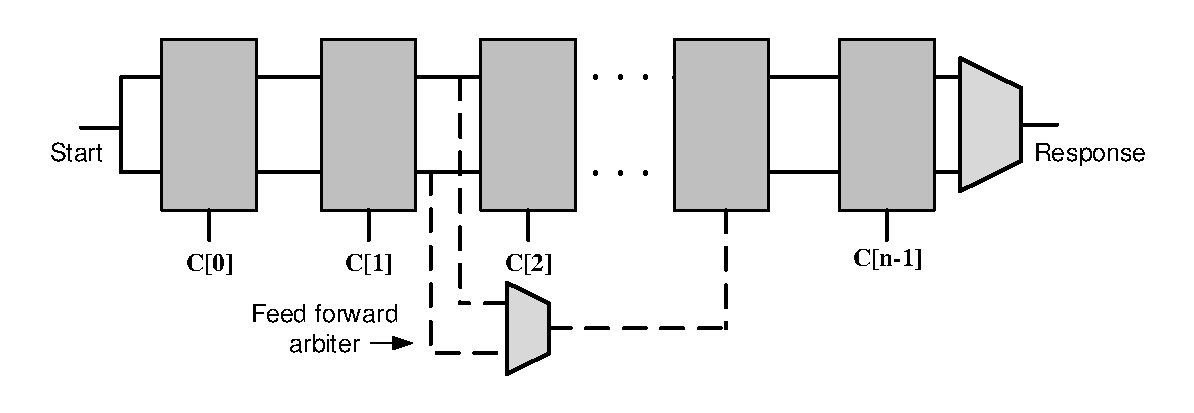
\includegraphics[width=\linewidth]{feedforwardpuf}
\caption{前馈仲裁型 PUF}
\label{fig: ffpuf}
\end{figure}

但\parencite{lim2005extracting}中同样提到了 FFPUF 的攻击方法,而且可以在有限时间内完成,说明这种方法或单独使用这种方法仍是不安全的。

\subsection{异或输出的PUF}\label{subsec:xormethod}

\parencite{suh2007physical}中, G. Edward Suh 和 S. Devadas 提出了 XOR PUF,即是将采用多个传统仲裁型 PUF,给予相同的激励,并且将响应值全部异或起来。异或运算具有非线性特性,具体来讲,两个同激励的 PUF 异或之后输出可以表达成:
\begin{equation}\label{eq:xor-model}
R=p'd\times p'e
\end{equation}
d, e 分别代表两个 PUF 的内在参数,若要使R线性可分,必须要写成 $ P’D $ 的形式,将式\ref{eq:xor-model}展开可以写成 $ P’D $ 的形式,但在这里$ D $是 $ \frac{n(n-1)}{2} $ 维的向量, SVM 的计算复杂度由n上升到了 $ n^2 $,经过多个 PUF 异或后可以将运算复杂度上升到不能在有限时间尺度上求解。

异或的非线性特性不依赖于具体的 PUF 形式,因此是一种通用的增加 PUF 安全性的做法。但是异或的缺点显而易见:面积资源开销增加了N倍,同时误码率也增加了。

\subsection{双稳态环路PUF}
2011年Qingqing Chen等人在会议 Hardware-Oriented Security Transaction 上提出了一种新的PUF,双稳态环路型 PUF(Bistable Ring PUF,如图\ref{fig: brpuf})。  BRPUF 采用了偶数级反相器级联构成回路具有双稳态的特性构建 PUF 的观测点,具有新颖性,并且作者声称其环路具有非线性结构,较传统仲裁型 PUF 安全性更高\supercite{chen2011bistable}。

截止本文撰写时,仅有 Qingqing Chen 本人在文献\parencite{chen2012characterization}中对 BRPUF 做了特性分析; D. Schuster 和 R. Hesselbarth 对 BRPUF 用单层神经网络进行建模\supercite{schuster2014evaluation}。

\begin{figure}[htb!]
\centering
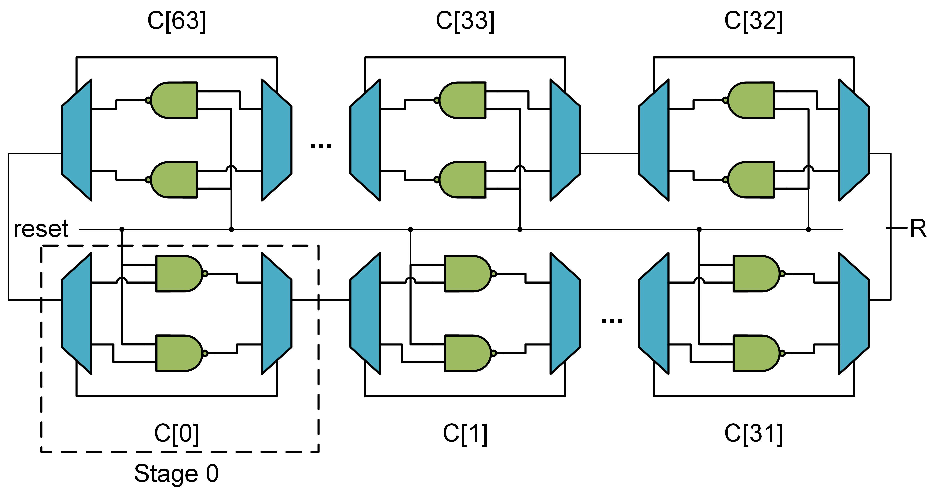
\includegraphics[width=\linewidth]{BRPUF}
\caption{双稳态环路型PUF}
\label{fig: brpuf}
\end{figure}

\section{本章小结}
本章介绍了 PUF 工作机制, PUF 的评价标准;介绍了针对 PUF 的机器学习建模攻击算法;以及列举了近期相关研究者的工作。 PUF 适合生成片间无关的大量激励-响应数据对,且占用资源和功耗相较于传统电路非常小,适合于物联网移动端芯片的内嵌安全模块。
但是目前 PUF 面临建模攻击的威胁,强大的机器学习算法可以用很小的代价推算出 PUF 的所有信息,这样致使一般的 PUF 原型设计不能直接应用于工程芯片。大量的研究者给出了新的设计方案,在下一章中,本文将对其中一个设计进行分析,并提出 PUF 设计的指导性标准。

	% vim:ts=4:sw=4
% Copyright (c) 2014 Casper Ti. Vector
% Public domain.

\chapter{基于PUF建模的仿真分析和设计方法}\label{chap:buildingmodel}
\section{双稳环路PUF的建模分析}\label{sec:brpufmodel}

上一章中介绍了双稳态环路 PUF(BRPUF),在本章节中我们将对 BRPUF 建模分析,指出在电路结构上影响 PUF 输出分布的几个因素。

\subsection{偶数级环路振荡器}

BRPUF 的一个单元包含了两个选择器和与非门,整体延迟比较大,而仿真发现,延迟较大的反相器构成的偶数级环路并不会迅速稳定。

\begin{figure}[htb!]
\centering
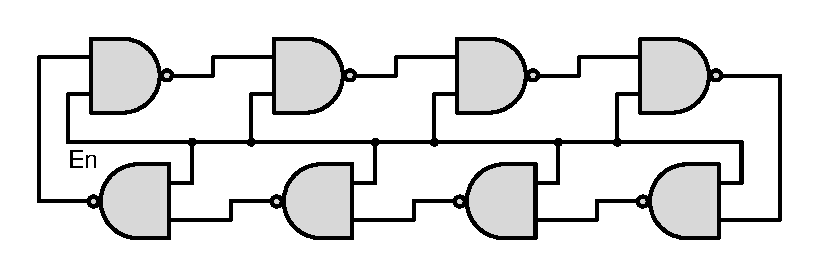
\includegraphics[width=\linewidth]{bistable-ring}
\caption{偶数级环路}
\label{fig:bistable-ring}
\end{figure}

\begin{figure}[htb!]
\centering
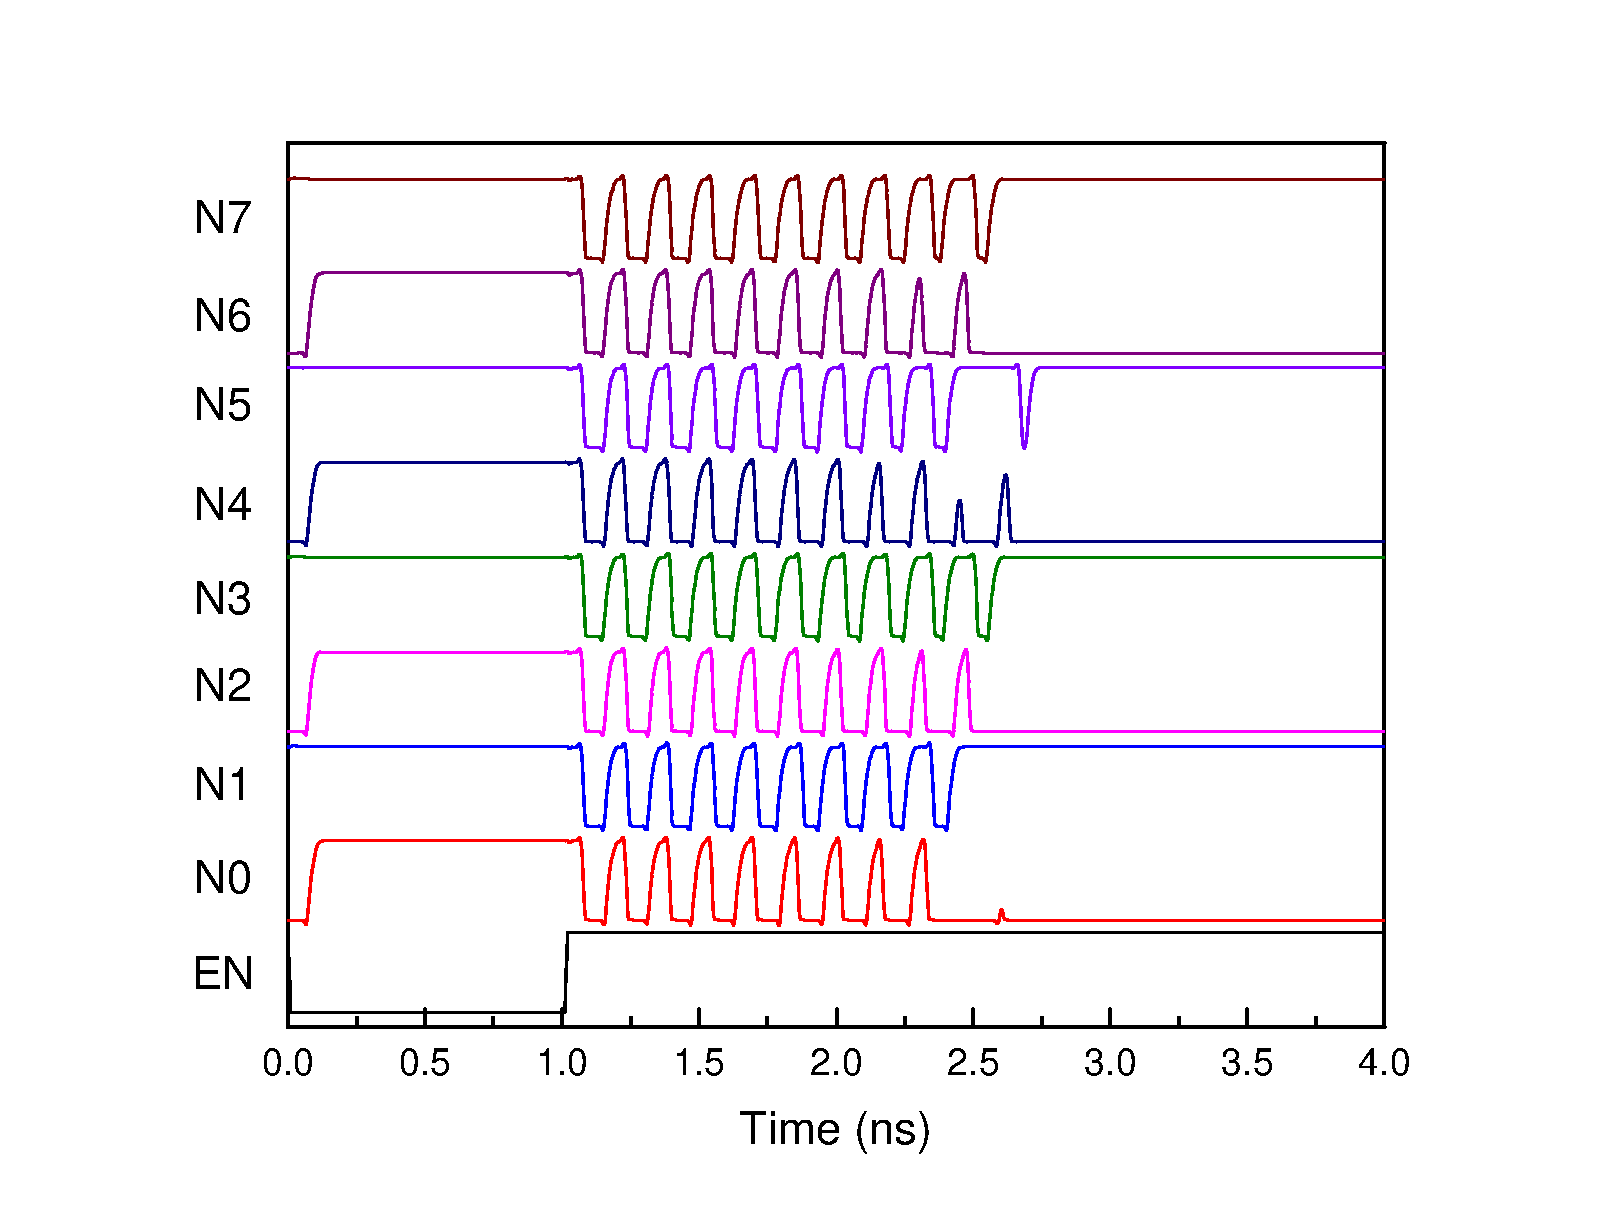
\includegraphics[width=\linewidth]{br_waveform}
\caption{偶数级环路仿真波形图}
\label{fig:brwaveform}
\end{figure}

如图\ref{fig:bistable-ring}所示,环路由$ N=8 $个与非门组成,当EN信号为低时,所有节点处于充电状态,当EN信号上跳时,电路开始进入``震荡状态''(如图\ref{fig:brwaveform}所示)。由于每个与非门的延迟时间远大于信号的上升时间和下降时间,故建立如下的模型:

\textbf{定义1:}第i个与非门的0-1上升延迟为$ tr_i $,1-0下降延迟为$ tf_i $。

当一个占空比为W的方波通过与非门i后,输出方波占空比变为:
\begin{equation}
W_{i+1}=W_i+\frac{tf_i-tr_i}{T}
\end{equation}
其中T为方波周期。当EN信号上跳后,初始占空比为$ W_0 $的方波激励输入与非门i,输出占空比为$ W_1 $,动态的考虑这个方波,当它经过N个与非门驱动后环回初始的节点,其占空比变为:
\begin{equation}
W_N=W_0+\sum\limits_{i=0}^{N}\frac{(-1)^i(tf_i-tr_i)}{T}=W_0+\Delta W
\end{equation}
当 $ \Delta W>0 $ ,则占空比趋向于1,意味着i与非门的输出节点最终收敛到逻辑``1'',反之则说明i与非门输出节点收敛到逻辑``0''。当 $ \Delta W=0 $ 时,占空比不发生变化,只要在一个环回周期内占空比不会变为1或0,那么电路将``理想''得 振荡下去,因此称其为偶数级环振。

\textbf{定义2:}环路中信号周期定义为所有逻辑门延迟之和。节点k的一次震荡(1次下跳和1次上跳)称为一个子周期。

\textbf{推论1}:N级环路(如不特别说明,此后环路中N为偶数)如不收敛,一个信号周期内节点k经历N/2个子周期;

\textbf{推论2}:偶数级环振振荡次数 $ M \propto \frac{W_0}{\Delta W}\cdot\frac{N}{2} $ ,故与非门上升下降延迟之差越小,延迟差总和越小,振荡次数越大。

振荡次数会影响 BRPUF 的求值时间,而且越久的振荡越容易收到噪声扰动使得电路不能在求值周期内收敛或者随机收敛。

\subsection{BRPUF模型}\label{subsec:brpufmodel}
接下来考虑图\ref{fig: brpuf}中的 BRPUF 电路,记激励 $ c_i\in{-1,1} $,一个单元内两个与非门的上升延迟和下降延迟分别为$ p,q,r,s $,取下标系数为0的与非门输出信号作为响应R。根据上一节分析知,响应R有:
\begin{equation}\label{eq:brmodel}
R=sgn(\sum\limits_{i=0}^{N}(-1)^i(\frac{1+c_i}{2}(p-q)+\frac{1-c_i}{2}(r-s)))=sgn(\sum(\alpha_i c_i+\beta_i))
\end{equation}
其中$ \alpha_i=(-1)^i\frac{p_i-q_i-r_i+s_i}{2} $, $ \beta_i=(-1)^i\frac{p_i-q_i+r_i-s_i}{2} $,类比\ref{subsec:apufmodel}节中的工作,可以将R写成
\begin{equation}
R=sgn(p'd)
\end{equation}
这是一个线性表达式,所以对于N级 BRPUF,则在N维空间中存在超平面可以将 CRP 区分开。在\ref{sec:modelverify}节中我们将演示用 SVM 拟合 FPGA 上的 BRPUF 参数向量d。

\subsection{BRPUF输出统计特性}\label{subsec:brpuf_stat}
在\ref{subsec:metrics}小节中介绍了 PUF 的几个评价指标,其中随机性、独特性和可靠性是 PUF 的统计特性,为了方便起见,定义工艺波动呈正态分布,故由工艺波动导致的单元延迟时间$ p,q,r,s $也近似呈正态分布。

\textbf{假设1:} BRPUF 单元延迟时间服从正态分布,即$ p,q,r,s \sim N(\mu,\sigma) $。

由 BRPUF 的模型式\ref{eq:brmodel}可知,$ R=sgn(\delta),\delta=\sum(\alpha c+\beta)=A'C+B $,则在随机性统计中,样本容量最大为$ 2^N $(N为激励位数),所以
\begin{equation}\label{eq:mean_delta}
\mu(\delta)=\frac{\sum A'C}{2^N}+B
\end{equation}
从0取到$ 2^N-1 $过程中,任意一位$ c_i $总是 一半为1, 一半为-1,所以式\ref{eq:mean_delta}前者之和为0,故有$ \mu(\delta)=B $。

同理可得
\begin{equation}
\sigma(\delta)=\frac{1}{2^{N/2}}\sqrt{\sum(A'C)^2}=\sqrt{\sum\alpha_i^2}
\end{equation}
\textbf{假设2:}PUF 芯片内各晶体管工艺波动分布类似,可令$ p,q,r,s $服从正态分布的均值和标准差相等,即对$ \forall i,\mu(p_i )=\mu(q_i )=\mu(r_i )=\mu(s_i )=\mu_i,\sigma(p_i )=\sigma(q_i )=\sigma(r_i )=\sigma(s_i )=\sigma_i $。

由B的表达式可得:
\begin{equation}
B\sim N(\mu_B,\sigma_B)
\end{equation}
\begin{equation}
\mu_B=\sum\mu(\beta_i)=0
\end{equation}
\begin{equation}
\sigma_B=\sqrt{\sum\sigma^2(\beta_i)},\sigma(\beta_i)=\dfrac{\sqrt{\sigma^2(p_i)+\sigma^2(q_i)+\sigma^2(r_i)+\sigma^2(s_i)}}{2}=\sigma_i
\end{equation}
故B的分布均值为0,标准差是单个单元延迟标准差的$ \sqrt{N} $倍。

对于单个 PUF 芯片的随机性统计,若B严格为0,则随机性严格地为50\%。若要求随机性的下限不得低于$ Rn_L $,上线不得高过$ Rn_H $,根据统计学知识,$ Rn=\frac{1}{2}erfc(x) $,其中 erfc 是余误差函数,$ x=-\frac{B}{\sqrt{2}\sigma(\delta)} $。故设一个 BRPUF 芯片随机性Rn满足条件的概率为P:
\begin{equation}
P=\int\limits_{Rn_L}^{Rn_H}\dfrac{Rn\cdot dx}{\int\limits_{-\infty}^{+\infty}Rn\cdot dx}
\end{equation}
根据 Matlab 的模拟,$ \mu(\delta) $的分布的标准差与$ \sigma(\delta) $的分布标准差比值$ \frac{\sigma(\mu(\delta))}{\sigma(\sigma(\delta))} $ 越大, Rn 分布的尖峰越高,比值为1时 Rn 呈随机分布,比值小于1, Rn 呈谷型分布。由假设2, BRPUF 的比值接近于1,故P近似于$ Rn_H-Rn_L $。

根据 PUF 独特性的定义,Rn接近50\%的概率越大,独特性越接近50\%;反之,说明多个 PUF 中大量个体输出分布偏差很大,个体之间汉明距离跟趋向于0和N两个极限值。

而可靠性主要考虑$ p,q,r,s $随环境变化对$ sgn(\delta) $的影响。

综上我们得到: BRPUF 的随机性和独特性较低。


\section{基于统计分析的PUF设计方法}
可以将\ref{sec:brpufmodel}节的分析推广开。第一代PUF\footnote{\parencite{rostami2014quo}中对PUF的总结,区别于Digital PUF}由3部分组成:物理信息转换模块,仲裁模块和输出模块。

若输出数字电路信号,则物理信息转换模块一定能写成 $ p’d $ 的形式,但 p,d 向量的维度不一定是激励的位宽,维度越大,说明转换过程越复杂;在上面的几个例子中,仲裁模块都是 sgn 函数,实际上任何二值逻辑输出都能等价为 sgn 函数;输出模块取决于整体系统设计,可以异或多个 PUF 的响应,也可以添加投票机制以提高稳定性\supercite{mathew201416}。

由\ref{sec:brpufmodel}节讨论可知, PUF 随机性Rn与 $ \frac{\sigma(\mu(\delta))}{\sigma(\sigma(\delta))} $ 相关,且比值应越大越好。

PUF 的随机性分布与独特性有关联,两个独立 PUF 元件的随机性分别为$ Rn_1,Rn_2 $,则两个 PUF 由N个随机激励产生的响应 R1,R2 的汉明距离 HD 有:
\begin{equation}
N|Rn_1-Rn_2|\leq HD\leq N\times min{Rn_1+Rn_2,2-Rn_1-Rn_2}
\end{equation}

推导HD的分布相当复杂,本文仅根据Matlab仿真得到定性结论:
\begin{itemize}
\item 只要Rn分布的均值是0.5,则HD的分布是均值0.5的高斯分布;
\item Rn的方差越小,HD的方差也越小,反之HD的方差越大;
\item Rn的方差与 $ \frac{\sigma(\mu(\delta))}{\sigma(\sigma(\delta))} $ 有关,比值越大,方差越大;
\end{itemize}

事实上上述比值的分母由工艺条件决定,在电路实际制造中往往希望工艺波动即分母越小越好,这不利于 PUF 的实现,所以 PUF 的设计应该在此基础上使转换值的均值分布方差越小。


\section{模型验证}\label{sec:modelverify}
\subsection{仿真验证}\label{subsec:simu}
仿真采用 HSPICE 和 Matlab 模拟结合的方法,因为单用 HSPICE 这类动态仿真软件难以在有限时间内模拟大量数据。根据H SPICE SMIC 40nm 的库文件,取栅长 L=40nm, PMOS 有源区宽$ W_p=200 $nm, NMOS 有源区宽$ W_n=120 $nm。提取出蒙特卡洛仿真的参数,经过10000次蒙特卡洛得到带负载的反相器和与非门延迟分布(如图\ref{fig:inv-delay},图 \ref{fig:nand-delay}所示)。

\begin{figure}[htb!]
\centering
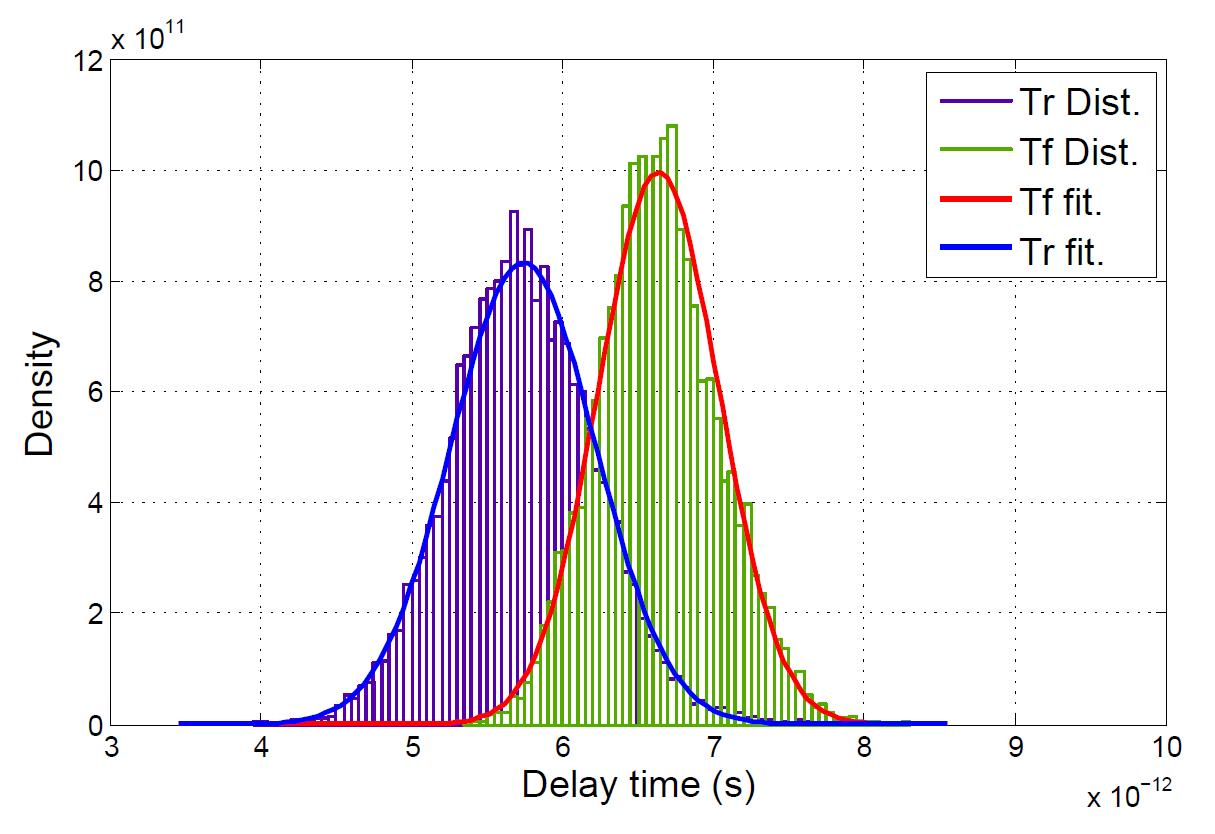
\includegraphics[width=.8\linewidth]{INV_Delay_Dist}
\caption{反相器延迟分布图}
\label{fig:inv-delay}
\end{figure}

\begin{figure}[htb!]
\centering
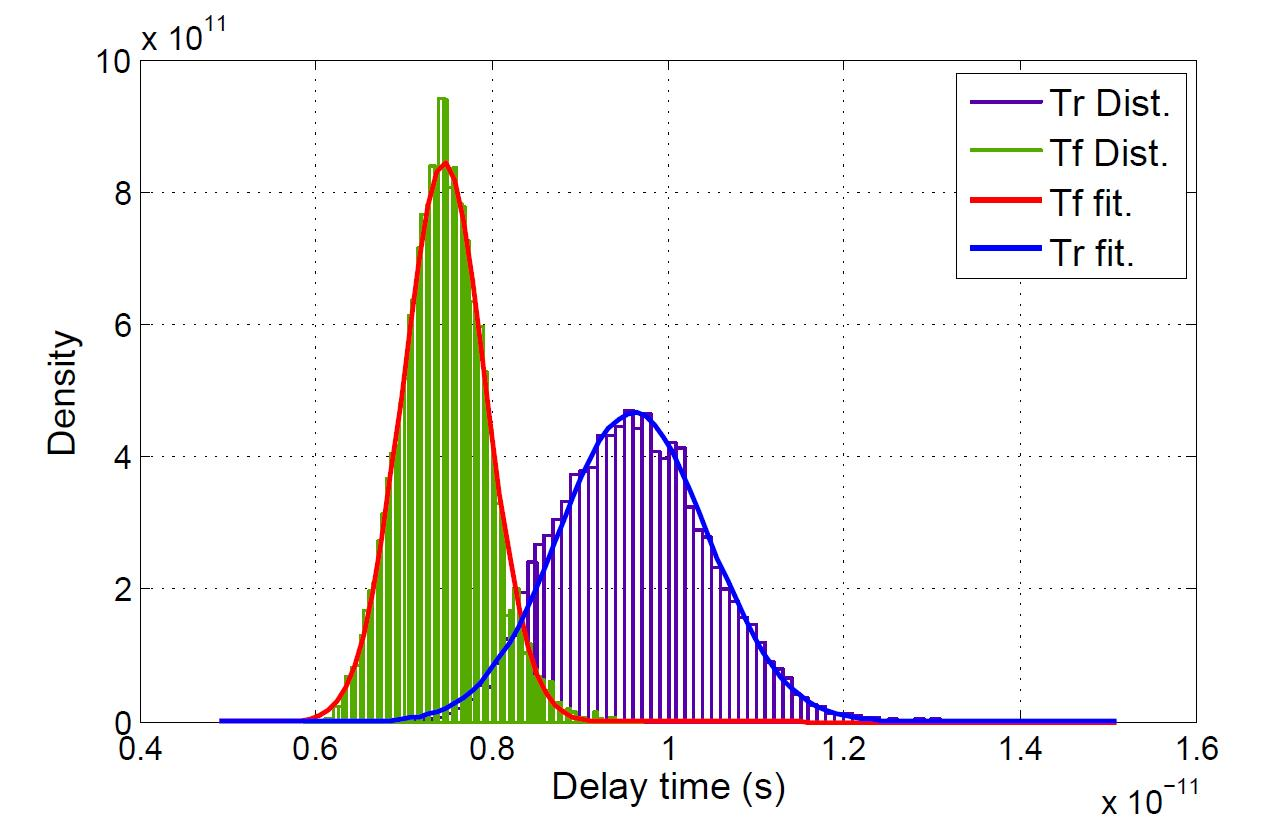
\includegraphics[width=.8\linewidth]{Nand_Delay_Dist}
\caption{与非门延迟分布图}
\label{fig:nand-delay}
\end{figure}

拟合出反相器延迟服从$ tr: N\sim(5.74\times 10^{-12},4.79\times 10^{-13}) $, $ tf: N\sim(6.64\times 10^{-12},4.00\times 10^{-13}) $,与非门延迟分布服从$ tr: N\sim(9.61\times 10^{-12},8.54\times 10^{-13}) $,$ tf: N\sim(7.46\times 10^{-12},4.72\times 10^{-13}) $,用 Matlab normrnd 函数生成一个 $ M\times 4 $ 的参数矩阵,其中4列分别代表每一级$ p,q,r,s $四个延迟参数,$ M $表示 BRPUF 的级数,这里取$ M=32 $。

将参数矩阵带入模型,按平均分布随机给定1000个32位激励值,得到1000位的响应向量。重复生成1000个参数矩阵(激励保持不变),最终得到一个$ 1000\times 1000 $的响应矩阵R。

由R的每一行求和除以$ M $可以得到一个随机性数值$ Rn_i $,任意两行之间做异或求和再除以$ M $,得到相对汉明距离$ HD_j $,HD的均值就是独特性Un,图\ref{fig:brpufrand},\ref{fig:brpufuniq}画出了 BRPUF 的 Rn 和 HD 的分布。

\begin{figure}[htb!]
\centering
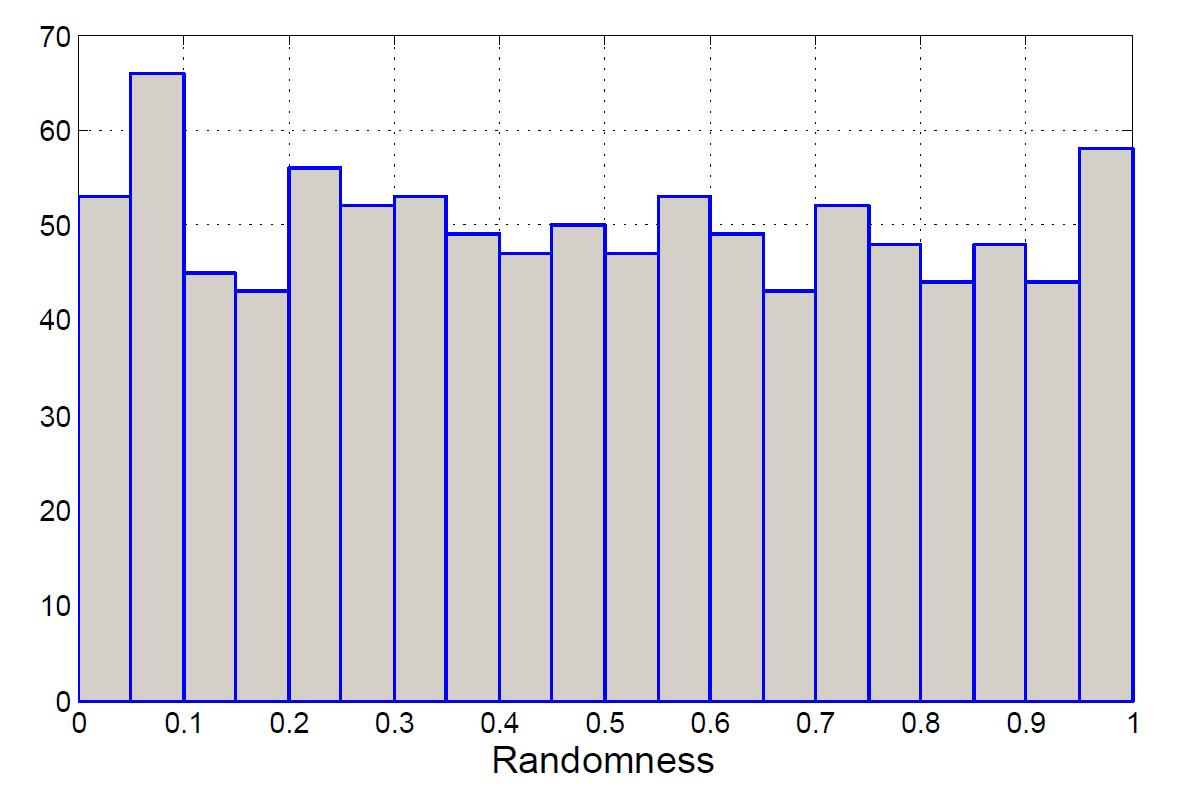
\includegraphics[width=.8\linewidth]{brpuf_rand_simulation}
\caption{BRPUF 随机性分布}
\label{fig:brpufrand}
\end{figure}

\begin{figure}[htb!]
\centering
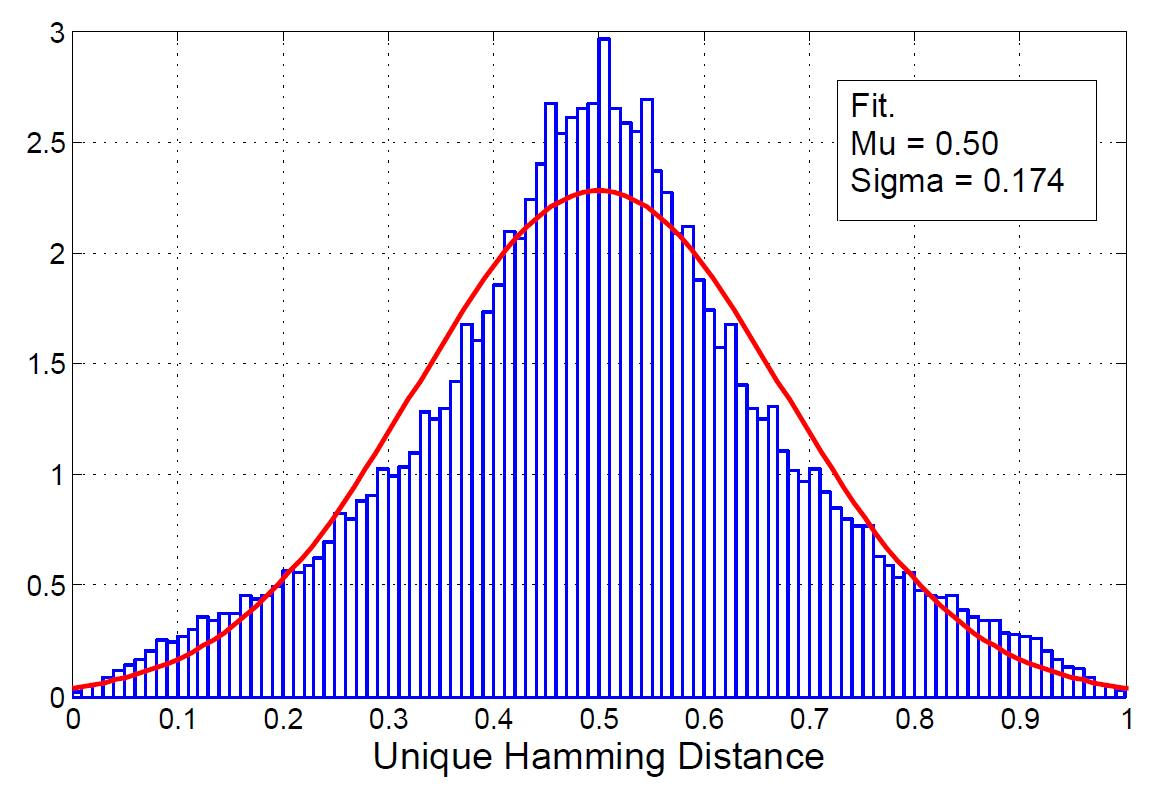
\includegraphics[width=.8\linewidth]{brpuf_uniq_simulation}
\caption{BRPUF 独特性分布}
\label{fig:brpufuniq}
\end{figure}

可以看到仿真结果和分析结论一致。 BRPUF 随机性的分布接近平均分布,独特性均值接近0.5但偏差较大,$ 3\sigma>0.5 $。

\subsection{FPGA验证}\label{subsec:fpga}
为了进一步验证理论分析结论,我们在 Altera Stratix V FPGA 芯片上实现了 BRPUF,其中一级单元用4个 LUT\footnote{Look Up Table,FPGA的基本逻辑单元} 实现,每个单元通过 Logiclock\footnote{逻辑锁定,Altera器件上固定LUT位置的工具} 固定在特定坐标的 LAB\footnote{Logic Array Blocks,由数个基本单元构成的逻辑块} 上,以保持布线平衡。读出逻辑通过 PCI-E 接口通信,在 PC 上给予激励和收集响应。并且根据 BRPUF 易振荡的特点,设定超时逻辑——以 250 MHz 时钟频率连续采样1000个输出,若连续100个保持恒定值则输出该值,否则认为没有在 $ 4\mu s $ 内收敛,输出 0xFF 表示该值无效。

我们在3块 FPGA 芯片上,每块放置30个 PUF,分别在不同的位置以模拟片间差异,一共90个 PUF,每个 PUF 收集1000个 CRP 。图\ref{fig:brpuffpga}展示了 Rn 和 HD 的分布。可以看出,用 FPGA 实现的 BRPUF 的输出分布与模拟分布一致,说明分析正确。

接下来根据模型将其中1个 PUF 的1000组 CRP 中的P\%用作 SVM 训练集($ P\leq 70 $),剩余固定30\%用于测试集,用 Matlab 的 fitcsvm 函数做 SVM 拟合。根据P的递增,得到预测准确率随P变化的图像,如图\ref{fig:svmfit}所示。

\begin{figure}[htb!]
\centering
\subfloat[随机性]{
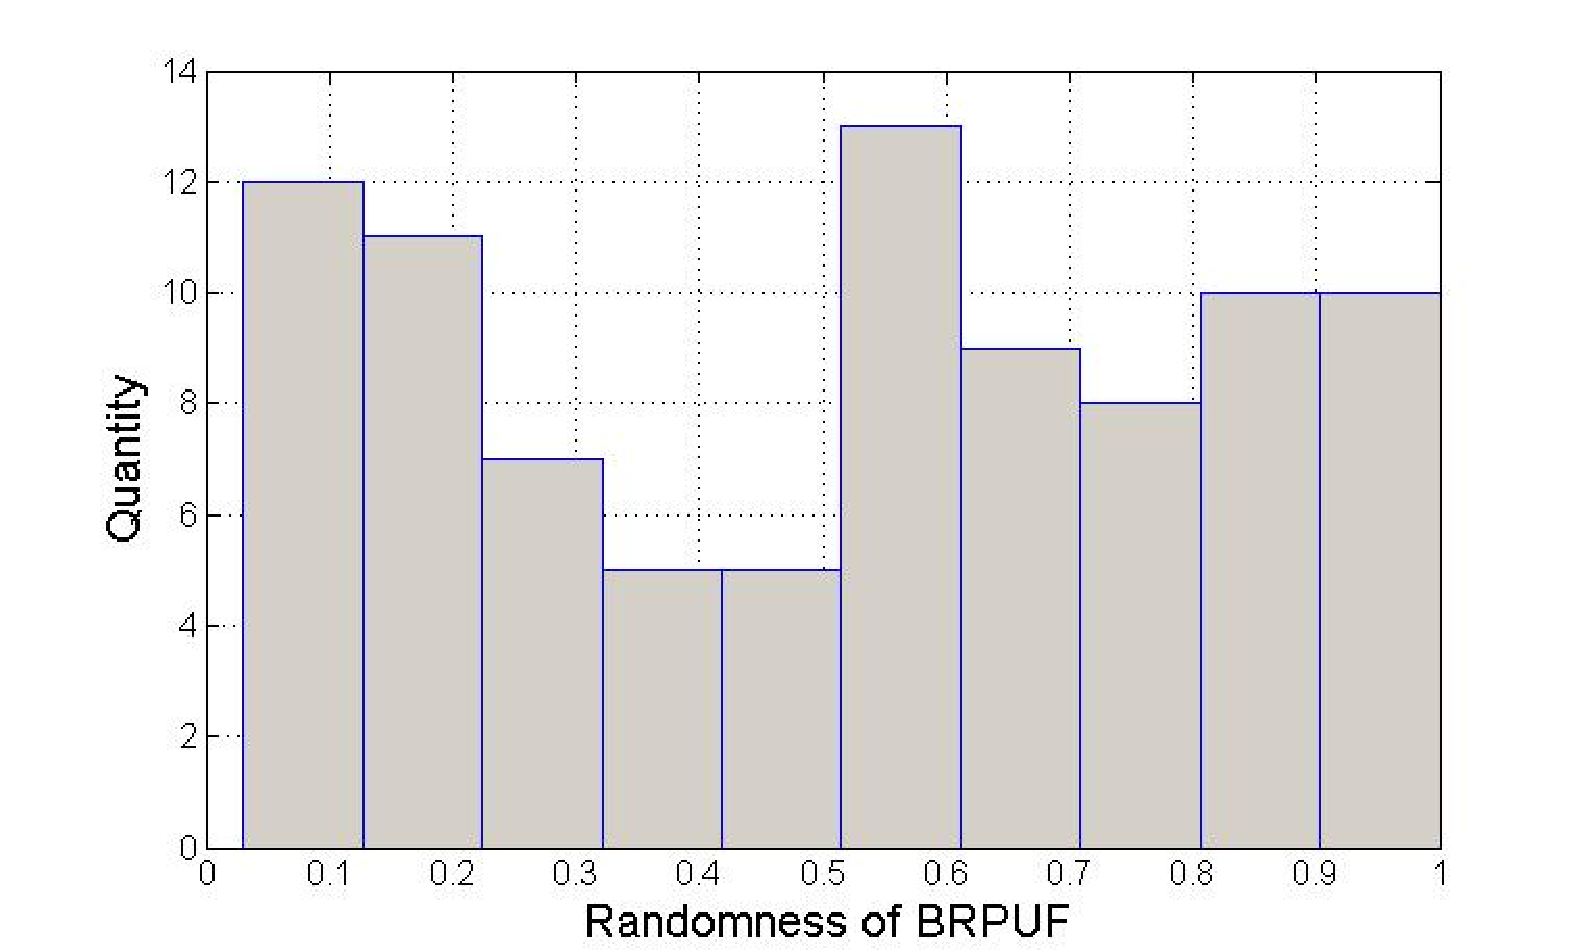
\includegraphics[width=.8\linewidth]{brpuf_rand_fpga}
}\\
\subfloat[独特性]{
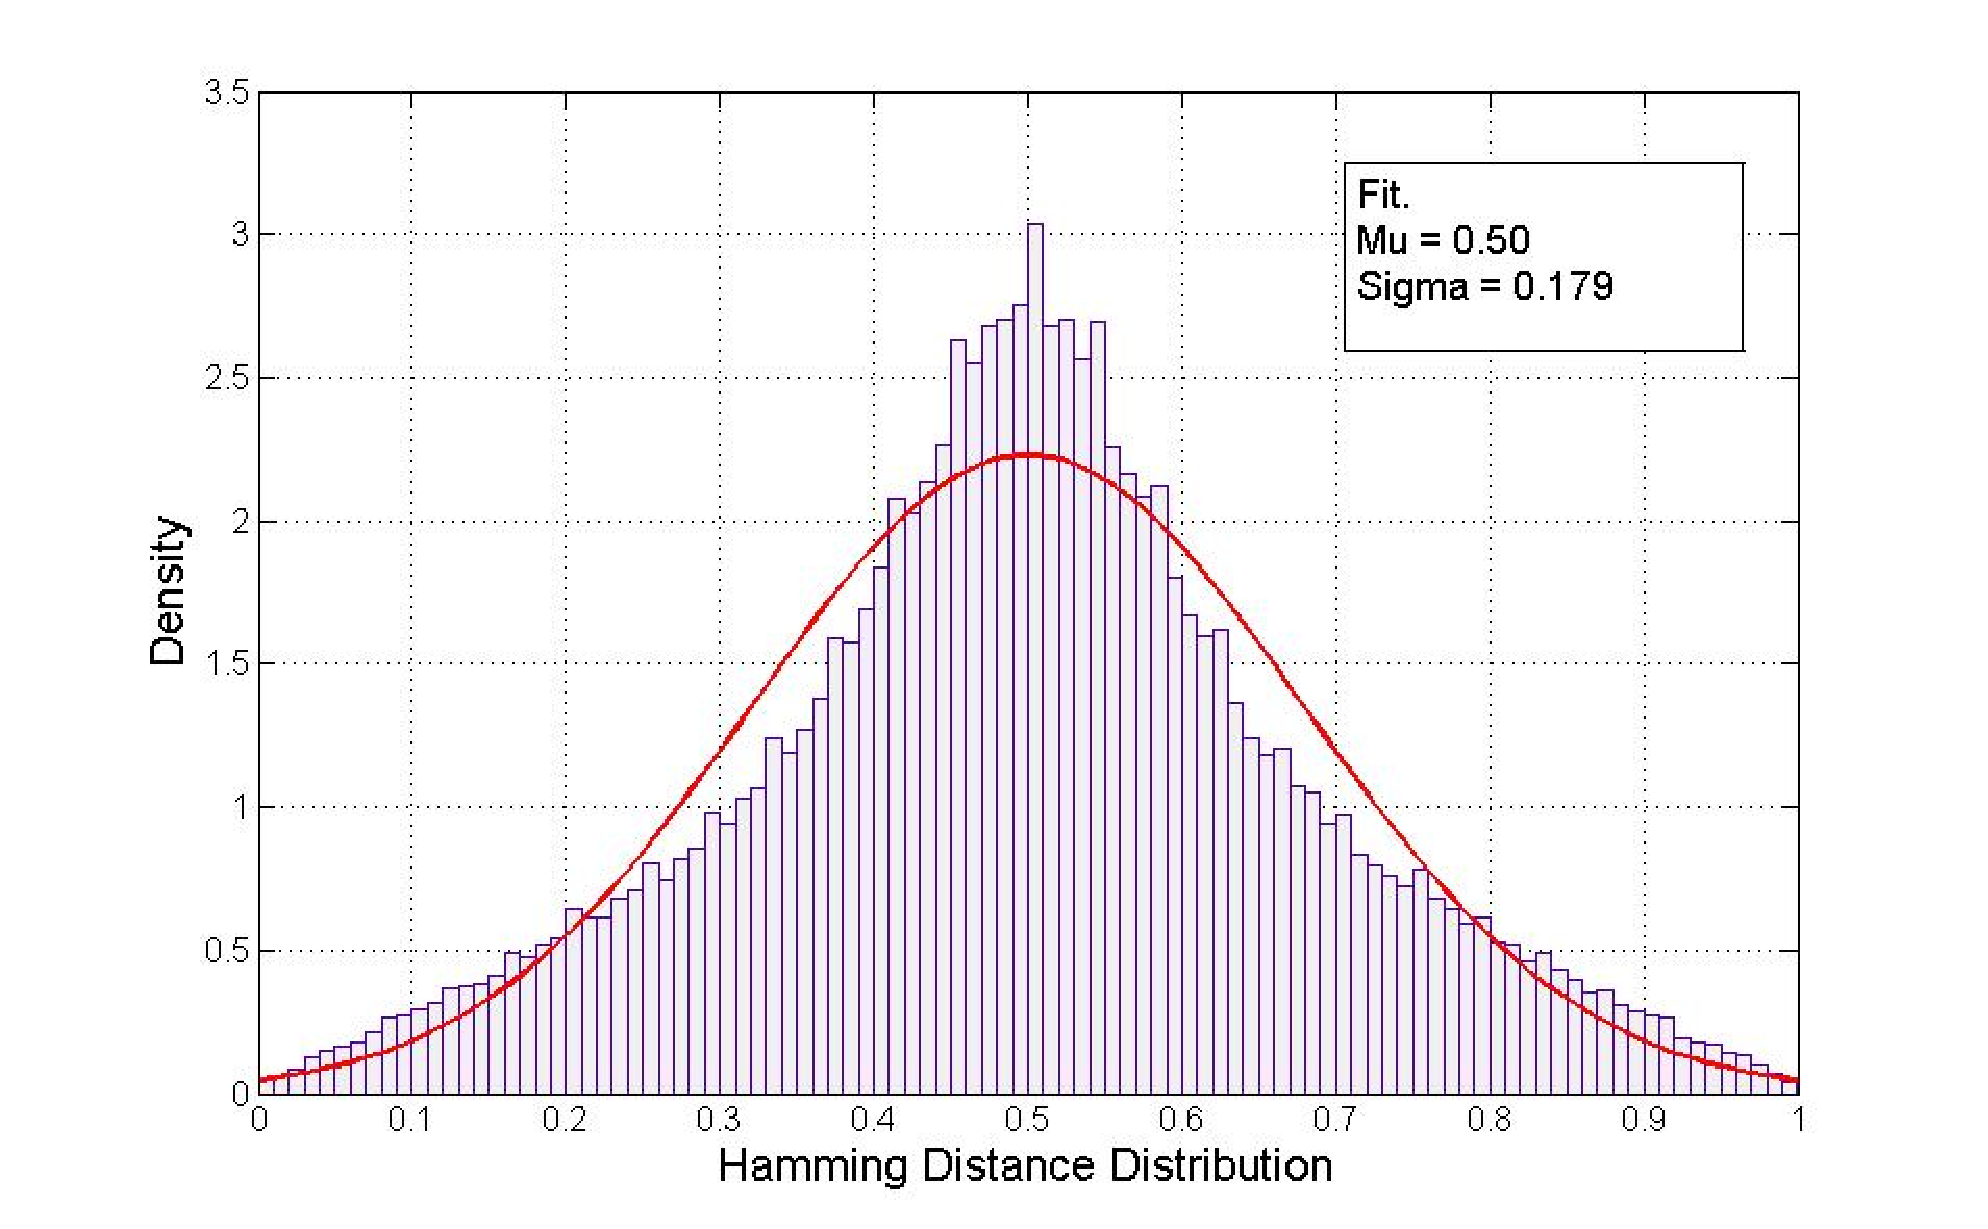
\includegraphics[width=.8\linewidth]{brpuf_uniq_fpga}
}
\caption{BRPUF FPGA实现分布}
\label{fig:brpuffpga}
\end{figure}

\begin{figure}[htb!]
\centering
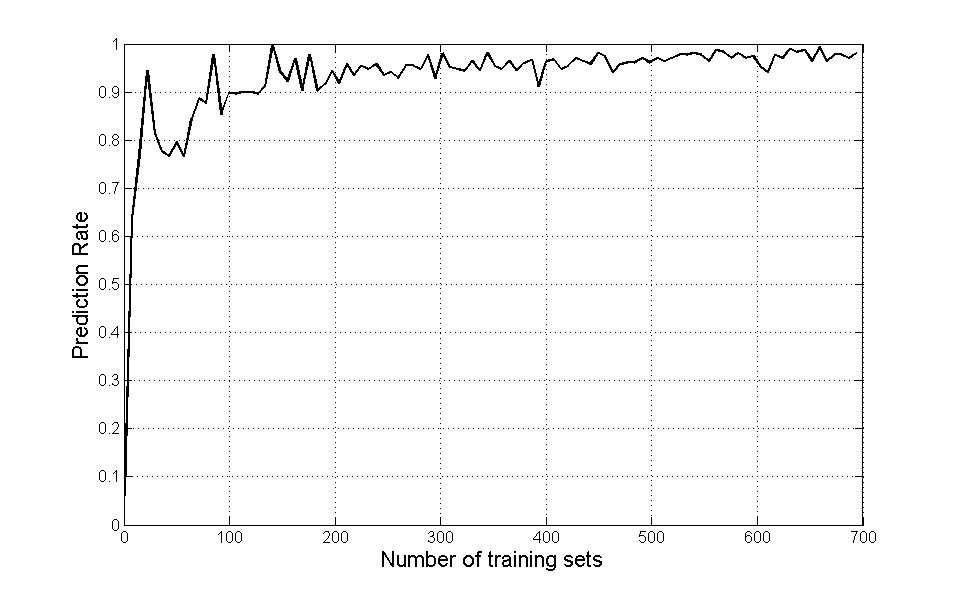
\includegraphics[width=\linewidth]{brpuf_fpga_svm.jpg}
\caption{SVM学习准确率}
\label{fig:svmfit}
\end{figure}

可以看出,预测率随训练集样本数上升的非常快,达到95\%以上的预测率仅需要200个训练样本,最终训练结果使得预测率超过99\%。

\section{本章小结}
在本章中我们首先对 BRPUF 进行了建模,根据模型分析了 BRPUF 的输出特性,由此指出其不足之处;其次提出了 PUF 在设计中遵循的原则,有利于在设计初期剔除分布较差的结构;最后通过 Matlab 和 FPGA 进行了验证并证明了我们的推论。
	% vim:ts=4:sw=4
% Copyright (c) 2014 Casper Ti. Vector
% Public domain.

\chapter{延迟环路PUF设计}\label{chap:dbrpuf}

\section{电路结构}\label{sec:dbrpuf_scheme}
从第\ref{chap:buildingmodel}章的讨论看出, BRPUF 输出分布扩散在(0,1)几乎呈均匀分布,这是 PUF 设计所不愿意看到的,其根本原因在于环路结构使得每一个环路中与非门的延迟波动产生叠加,造成了最终输出均值较大波动,在工艺方差不变的前提下,输出分布方差退化为工艺方差的N倍(N为级数),故N级数越高, BRPUF 输出分布越差。

结合 BRPUF 环路结构和仲裁 PUF 的延迟路径选择结构,提出了如图\ref{fig:dbrpuf}所示的电路,称为``延迟环路PUF''( Delay-based Bistable Ring PUF, DBRPUF )。

\begin{figure}[htb]
\centering
\includegraphics[width=\linewidth]{dbrpuf}
\caption{延迟环路PUF电路示意图}
\label{fig:dbrpuf}
\end{figure}

图\ref{fig:dbrpuf}所示结构由 $ N=2 $ 个单元构成,每个单元包含2个与非门和 $ K=4 $ 个双口交换器,其中交换器0\~2由激励 $ c_0\sim c_2 $ 控制,最后一级交换器由 $ z_0=c_0\oplus c_1\oplus c_2  $ 控制使得最后一级交换器的底输出端口一定与顶与非门I0联接,而顶输出一定与底与非门I1相联接,因此每个单元有 $ k-1 $ 位激励输入,1位信号输入,1位信号输出和1位复位信号。N个单元输入输出连接成环路,在此结构中,由 $ 2N $ 个与非门组成了双稳态环路,激励信号 $ c_i $ 控制每个与非门的延迟路径,根据\ref{sec:brpufmodel}节理论,双稳环路的稳定态与环路中每一个与非门延迟相关,图\ref{fig:dbrpuf}中延迟可以看成与非门本征延迟和交换器延迟的累积,因此改变交换器状态即改变了环路中与非门的输入信号延迟时间,进而导致电路进入不同的稳态。故该PUF结构的CRP共有 $ 2^{N(K-1)} $ 对。

\section{统计分析}\label{sec:dbrpuf_stat}
设第i个单元中顶与非门I0和底与非门I1的总延迟分别为 $ (Sr_i^T,Sf_i^T),(Sr_i^B,Sf_i^B) $,其中 $ Sr $ 代表总上升沿延迟, $ Sf $ 代表总下降沿延迟。令信号从顶与非门I0输出的时刻为 $ p_0 $ ,底与非门I1输出的时刻为 $ q_0 $。每一级交换器j有4条路径,每条路径有上升延迟和下降延迟两个变量,用 $ (x_0^j,x_1^j,x_2^j,x_3^j) $ 表示4条路径的上升沿延迟,同理用 $ (y_0^j,y_1^j,y_2^j,y_3^j) $ 表示下降沿延迟。

首先考虑上跳沿的传输。

\begin{eqnarray}
p_{j+1}=\frac{1-c_j}{2}(p_j+x_0^j)+\frac{1+c_j}{2}(q_j+x_2^j) \\
q_{j+1}=\frac{1-c_j}{2}(q_j+x_3^j)+\frac{1+c_j}{2}(p_j+x_1^j)
\end{eqnarray}

两式相减得到类似仲裁型PUF延时差的表达式

\begin{equation}
\Delta_{j+1}=p_{j+1}-q_{j+1}=-\Delta_jc_j+\alpha_jc_j+\beta_j
\end{equation}

两式相加得到:

\begin{equation}
S_{j+1}=p_{j+1}+q_{j+1}=S_j+\gamma_jc_j+\tau_j
\end{equation}

其中 $ \alpha_j=\frac{x_0^j-x_1^j-x_2^j+x_3^j}{2},\beta_j=\frac{x_0^j-x_1^j+x_2^j+x_3^j}{2},\gamma_j=\frac{x_0^j-x_1^j-x_2^j+x_3^j}{2},\tau_j=\frac{x_0^j+x_1^j+x_2^j+x_3^j}{2} $。

递推可以得到 $ \Delta_K, S_K $ 的表达式。而
\begin{eqnarray}
p_K=\frac{S_K-\Delta_K}{2} \\
q_K=\frac{S_K+\Delta_K}{2}
\end{eqnarray}

故I0传递到I1信号上升沿延迟 $ Sr_i^T=q_K-p_0 $,I1传递到输出端口的上升沿延迟 $ Sr_i^B=p_K-q_0 $。

同理可得,下降沿延迟具有相同的表达式,只是式中变量含义不同。

根据双稳态环路的稳定判据,可推出:

\begin{equation}\label{eq:dbrpufmodel}
R=sgn[\sum\limits_{i=0}^{N}[(Sr_i^T-Sf_i^T)-(Sr_i^B-Sf_i^B)]]=sgn[\sum\limits_{i}^{N}(\Delta r_K-\Delta f_K+\Delta_0)]
\end{equation}

其中 $ \Delta r $ 具体指上升沿延迟差,$ \Delta f $ 指下降沿延迟差,$ \Delta_0 $ 是常数偏置,其物理意义是信号进入交换器的时刻差 $ p_0-q_0 $,我们希望没有偏置,即$ \Delta_0=0 $,而则可以通过合理布局布线达到。由于$ \Delta r $和$ \Delta f $具有相同的表达形式$ \Delta=P'D $,式\ref{eq:dbrpufmodel}可以变为:

\begin{equation}
R=sgn[\sum\limits_{i}^{N}P'_i(D_i^1-D_i^2)]=sgn[\sum\limits_{i}^{N}P'_iD_i]
\end{equation}

最终简化成了N个子单元中延迟差的和。与仲裁型 PUF 具有相似的形式。

令$ \delta=\sum P'D $,由\ref{subsec:brpuf_stat}节相关推论可知,$ \delta $的均值分布的方差由 BRPUF 的 $ N=32 $ 倍于单元延迟方差,缩小到 $ N=4 $ 倍,而 CRP 则由 $ N\times (K-1)=32 $ 保持与 BRPUF 一致。

\section{仿真验证}
采用 SMIC 40nm 工艺制程,用 HSPICE 库进行蒙特卡洛仿真提取延迟参数,再带入 Matlab 脚本生成模拟电路矩阵,得到$ 1000\times 1000 $的 CRP 矩阵。
表[]列出了电路参数;图\ref{fig:dbrpuf_dist}展示了改进的 DBRPUF 的随机性分布和独特性分布图。

\begin{figure}[htb!]
\centering
\subfloat[随机性]{
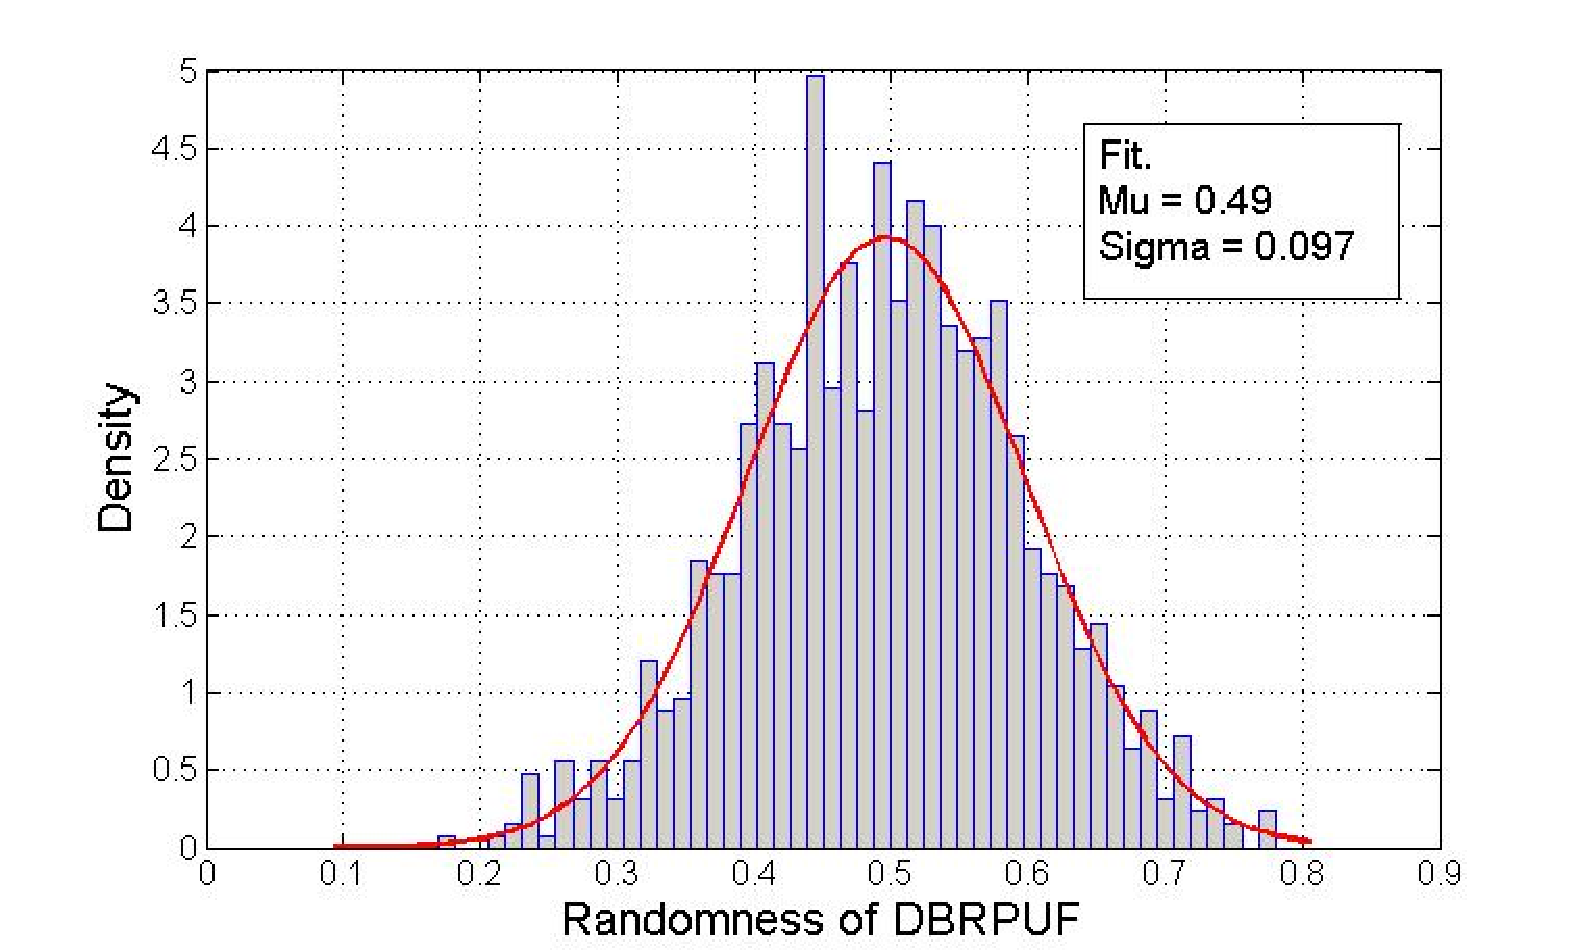
\includegraphics[width=.5\linewidth]{dbrpuf_rand_simulation}
}
\subfloat[独特性]{
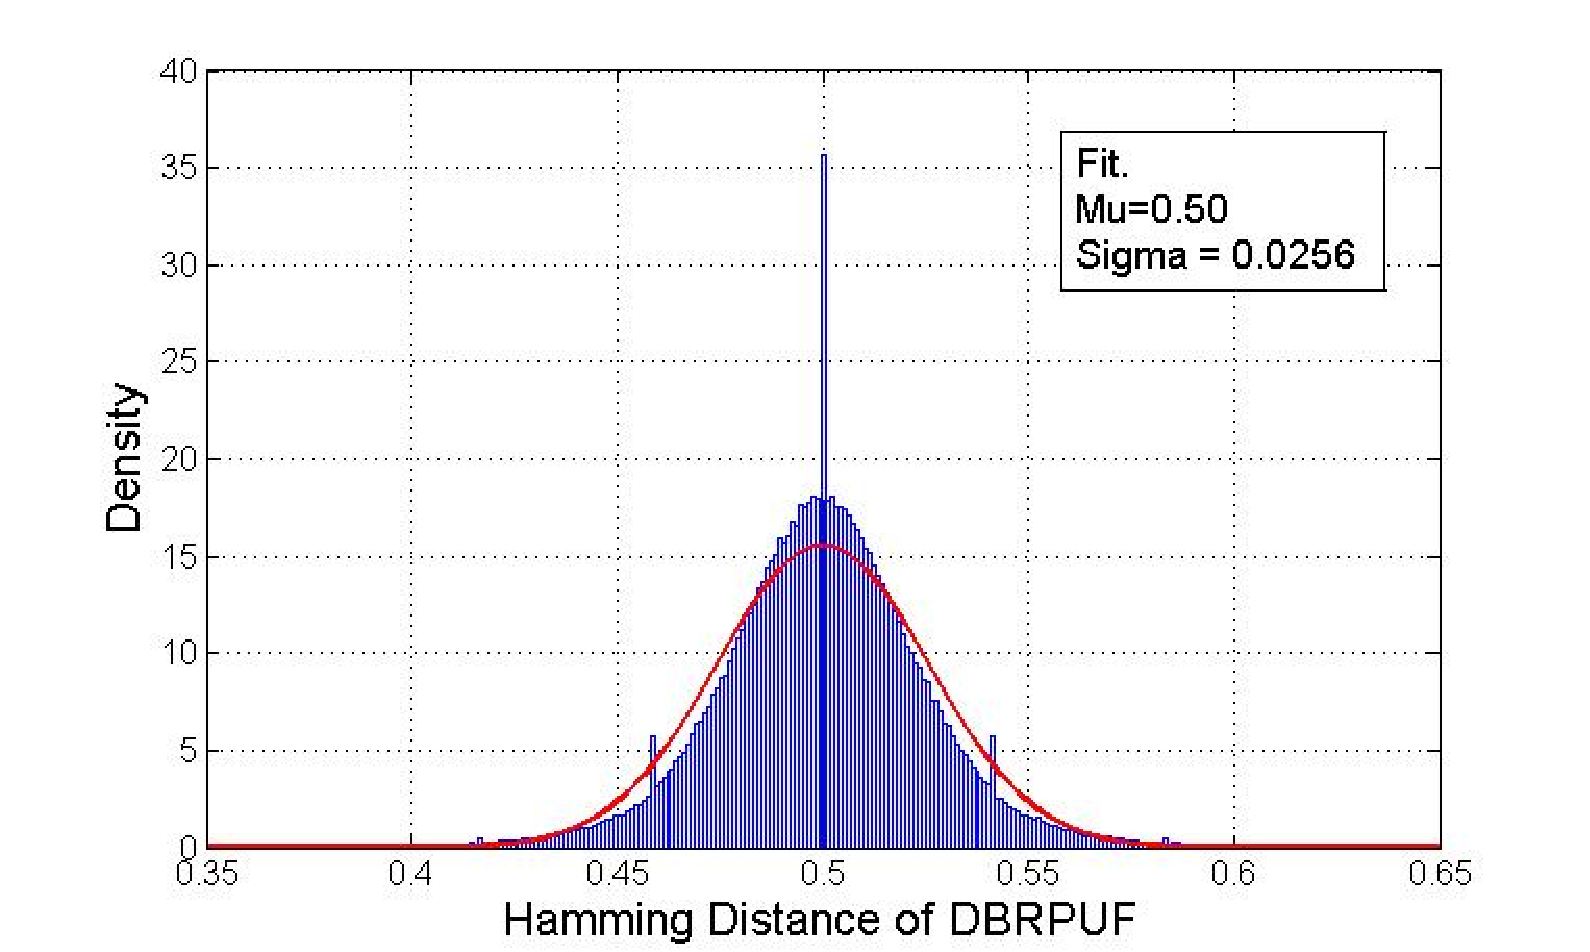
\includegraphics[width=.5\linewidth]{dbrpuf_uniq_simulation}
}
\caption{DBRPUF分布图}
\label{fig:dbrpuf_dist}
\end{figure}

可以看出 DBRPUF 的随机性分布达到 $ N_rand\sim(0.49,0.097) $,独特性分布达到 $ N_uniq\sim(0.50,0.0256) $,满足上小节的理论分析。相比于 BRPUF 大大改善了输出分布情况。但是 DBRPUF 的 CRP 仍然是n维空间线性可分,其复杂度与传统仲裁型 PUF 和 BRPUF 相当,为了提高模型复杂度必须采用多 PUF 单元异或的方式,无疑增加了电路的面积功耗开销,不利于 PUF 的实现。


\section{FPGA实现}
采用 Altera Stratix V 芯片,用3块 FPGA 综合并实现 DBRPUF 设计。图 17展示了 DBRPUF 实现的 Chip plan,我们用一个 LUT 实现交换器,故每一个单元级需要$ K+2 $个 LUT 实现$ K $个交换器和2个与非门。与 BRPUF 一样,需要手动设计 LUT 的摆放位置以保证布线的平衡。读出逻辑采用 250 MHz 时钟连续采样,若在 1000 个时钟周期内存在100个连续稳定的值则视其为输出,保存在输出寄存器中。寄存器的值和控制逻辑通过 PCI-E 接口与 PC 相连。

\begin{figure}[htb]
\centering
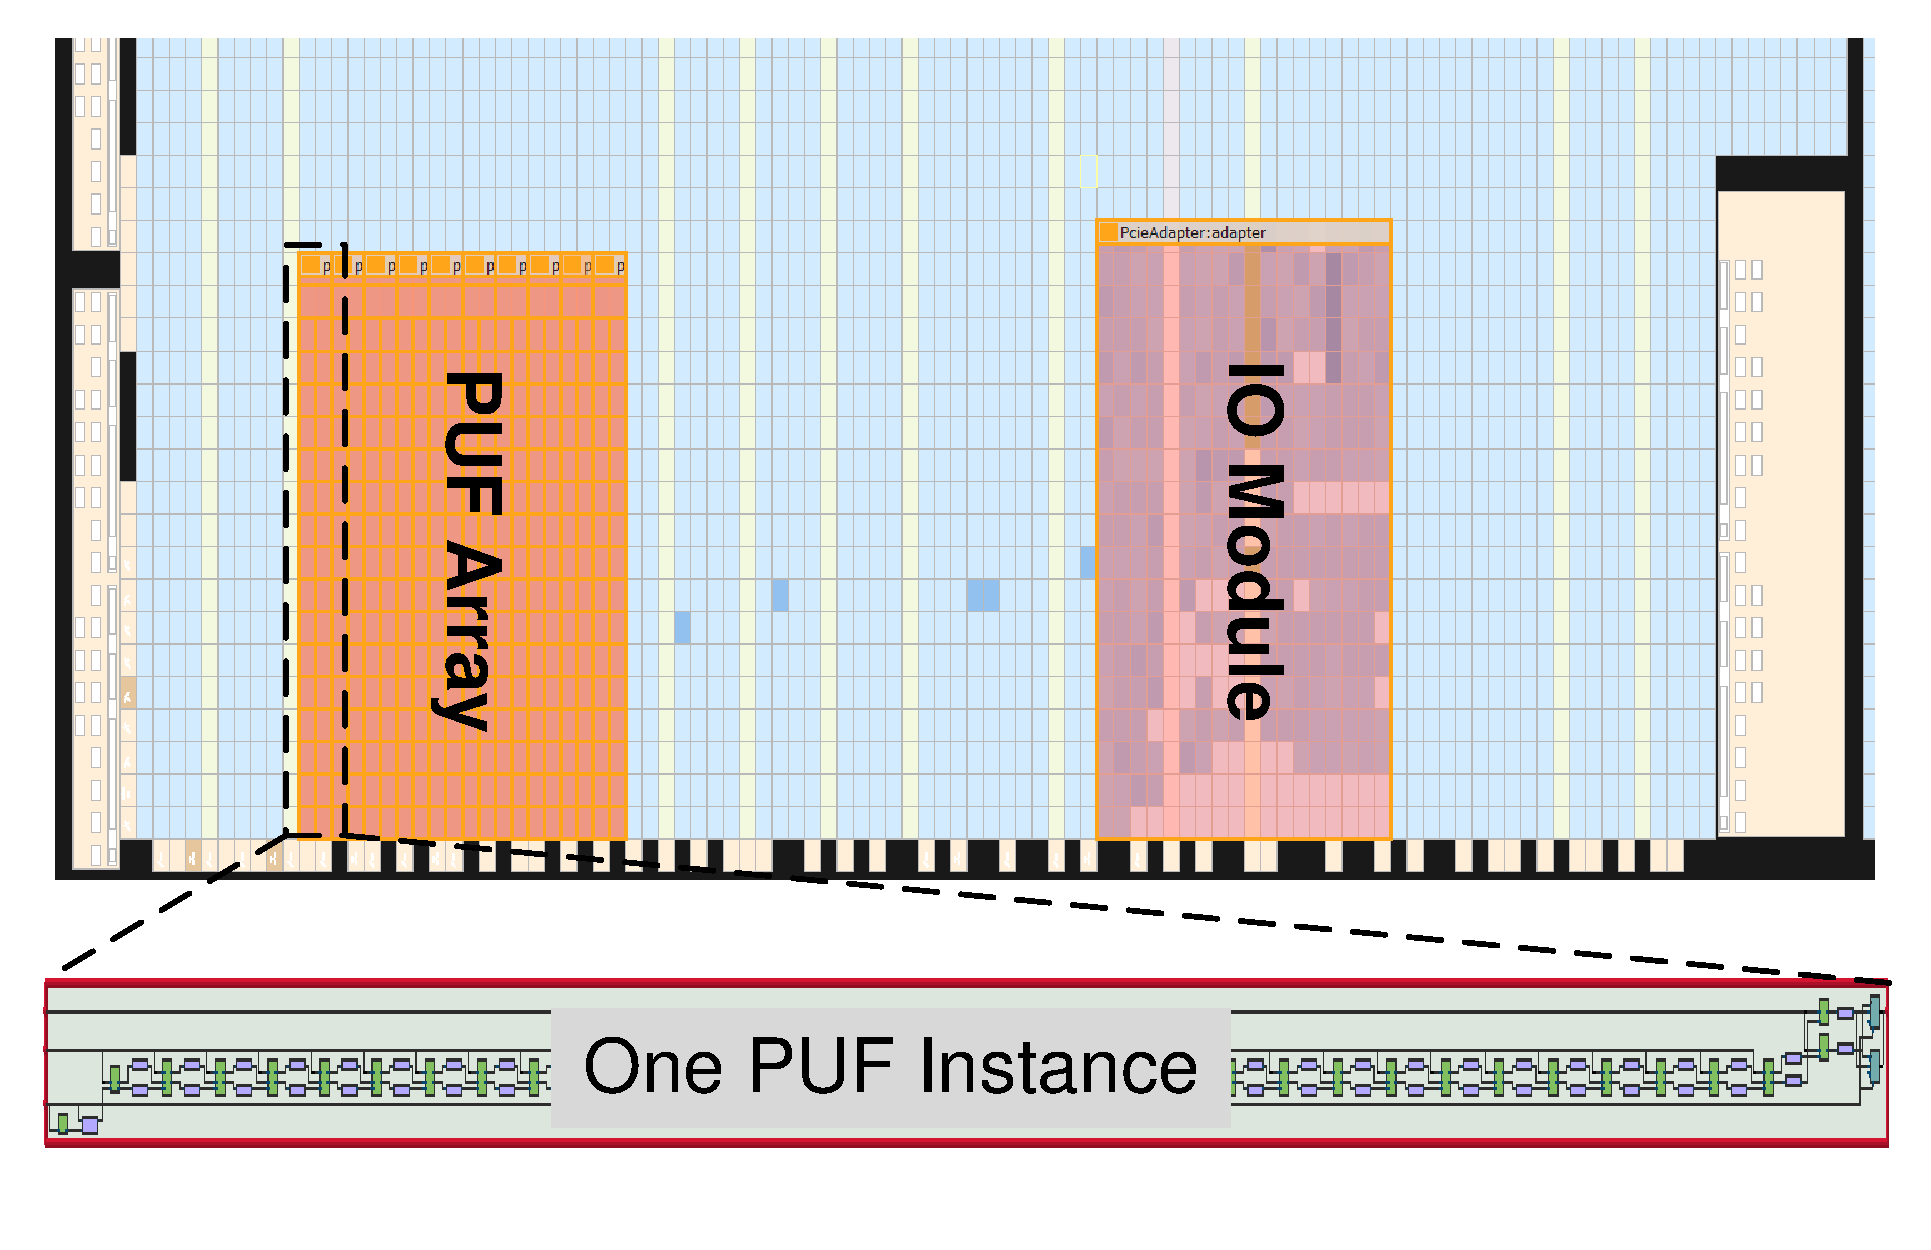
\includegraphics[width=.8\linewidth]{dbrpuf_cp}
\caption{DBRPUF在FPGA的Chipplan示意图}
\label{fig:dbrpuf_chipplan}
\end{figure}

在每块 FPGA 芯片的不同位置摆下10个 DBRPUF,共享一个读出逻辑,一共30个独立 PUF 元件。每个 PUF 等概率给予5000个随机32位激励,每个激励重复100次以验证可重复性,记录输出寄存器共 $ 30\times 5000\times 100 $ 个输出,经过 Matlab 统计分析,得到 DBRPUF 的随机性、独特性和可靠性分布。如图\ref{fig:dbrpuf_dist_fpga}所示, DBRPUF 的独特性满足 $ N\sim(0.494,0.0048) $ 的高斯分布,可靠性满足 $ N\sim(0.057,0.013) $ 的高斯分布(随机性样本太少不做统计)。

\begin{figure}[htb!]
\centering
\subfloat[FPGA随机性]{
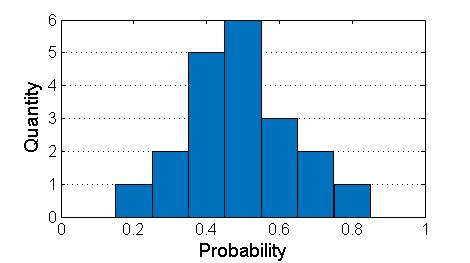
\includegraphics[width=.5\linewidth]{dbrpuf_rand_fpga}
}\\
\subfloat[FPGA独特性和可靠性]{
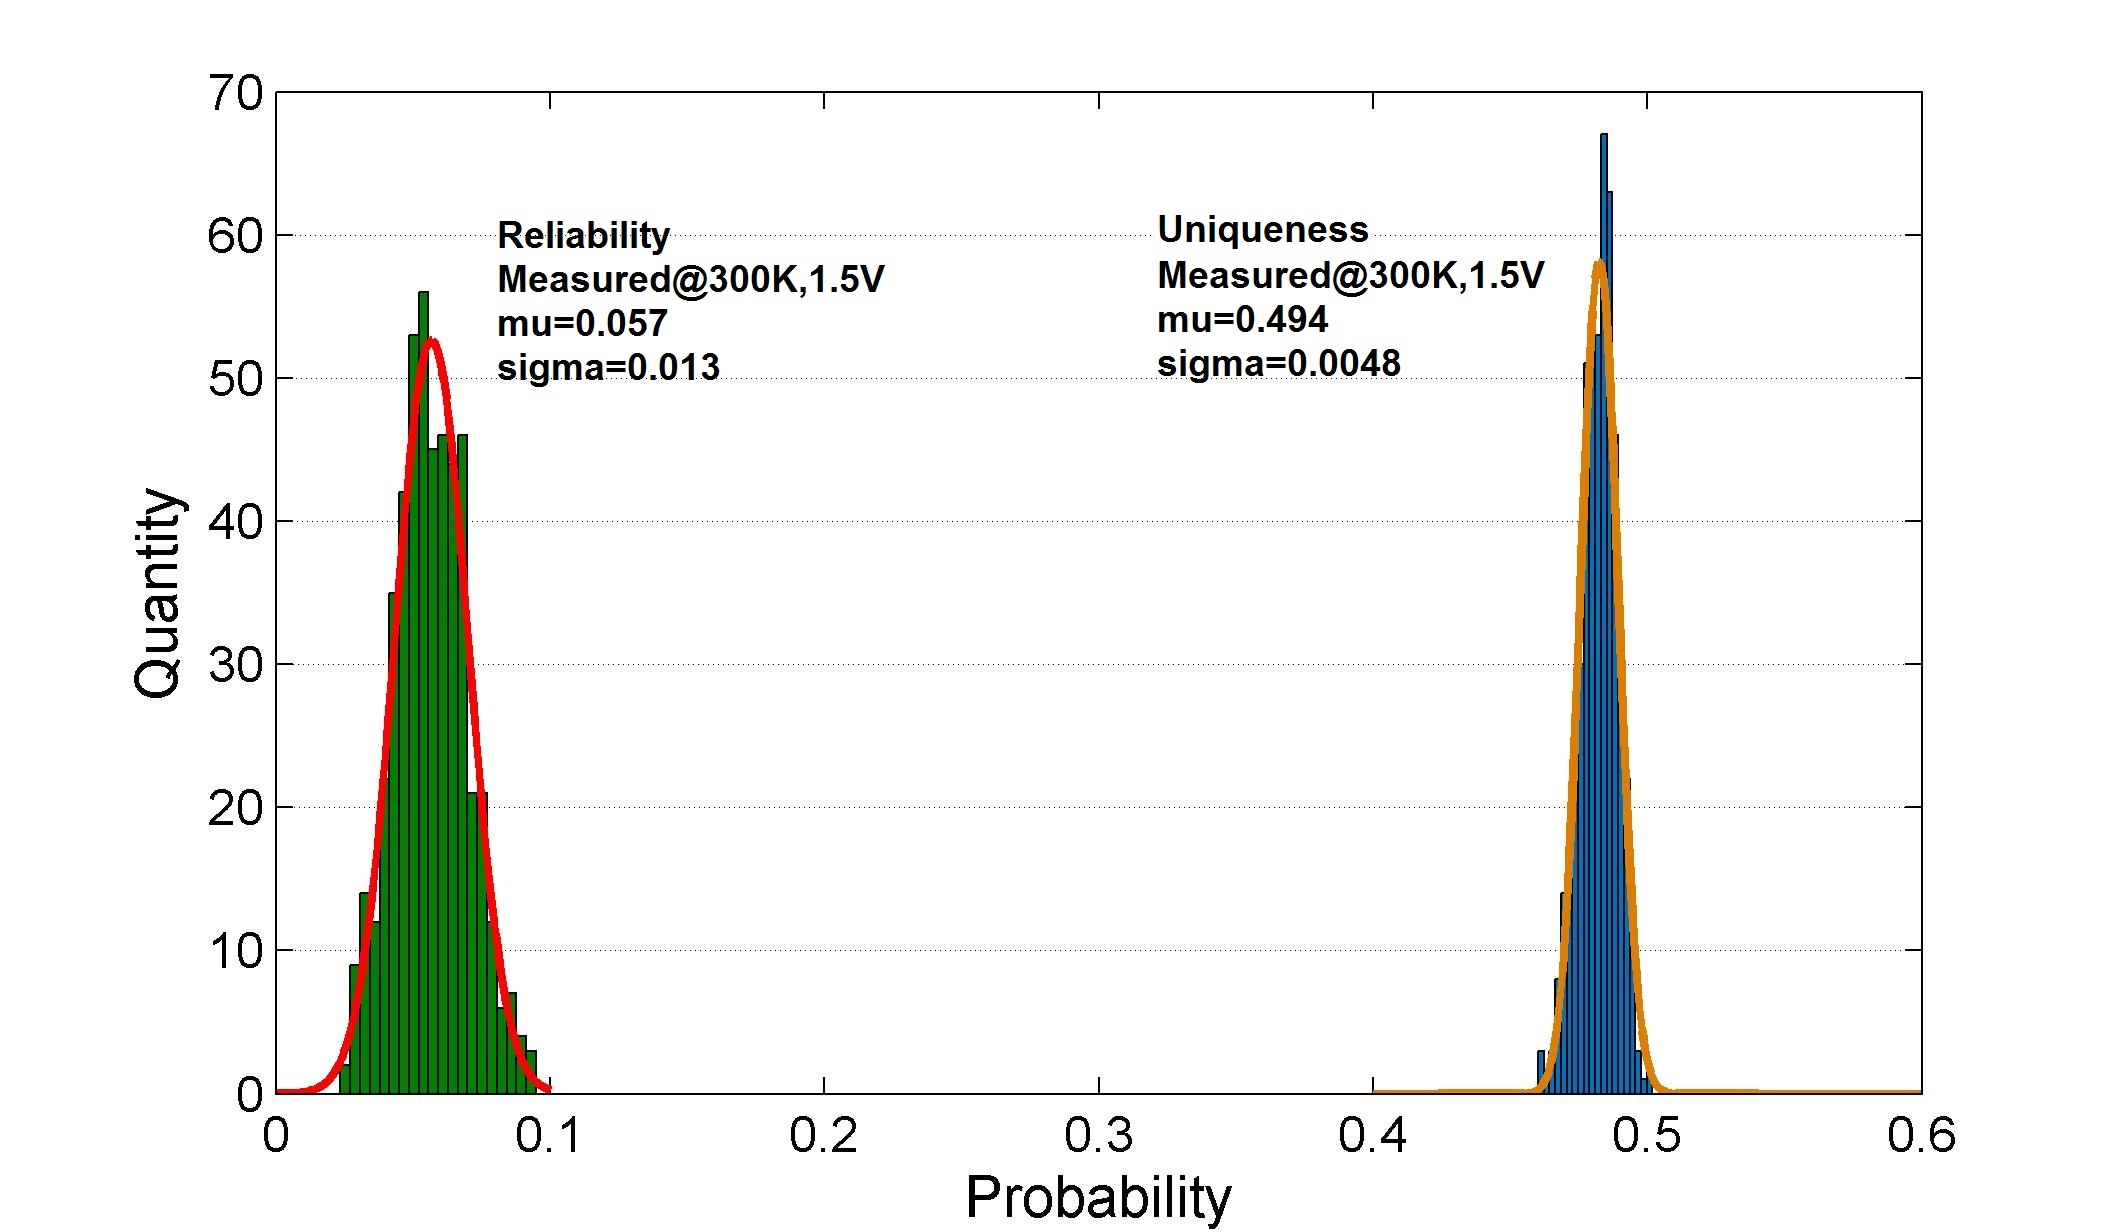
\includegraphics[width=.8\linewidth]{dbrpuf_uniq_fpga}
}
\caption{FPGA实现DBRPUF分布图}
\label{fig:dbrpuf_dist_fpga}
\end{figure}


\section{本章小结}
本章基于 BRPUF 和交换器设计了一种新型 PUF 结构,称为延迟双稳环路 PUF ( Delay-based Bistable Ring PUF )。
DBRPUF 改善了 BRPUF 分布分散的缺点,使得统计特性比 BRPUF 更好。并且从理论、仿真与 FPGA 三方面验证了这一结论。

但 DBRPUF 相比于传统仲裁型 PUF 并没有显著优势,其分布结果也没有达到最理想的效果,但是从 SVM 学习效果来看, DBRPUF 在一定程度上增加了学习复杂度,提高了求解时间代价。

	% vim:ts=4:sw=4
% Copyright (c) 2014 Casper Ti. Vector
% Public domain.

\chapter{随机脉冲仲裁PUF设计}\label{chap:rpapuf}
为了使 PUF 的安全性得到保障,统计分析和 NIST 测试通过是必要条件,尽可能提升模型复杂度也是必要条件。事实上,并不存在保证安全性的充分条件,因为总是有穷举的方法可以破解安全协议,而现有的攻击技术则是在一定时间成本下尽可能大的降低穷举复杂度。所以安全的攻和防是彼此的经济博弈,只有通过不断提升安全协议复杂度,同时又不增加系统开销,才能保证在相同经济能力下的相对安全性。

\ref{subsec:xormethod}节指出,多个 PUF 相异或可以提升总体模型的复杂度,将原N位 PUF 从 $ O(mn) $ 提升到 $ O(m'n^l) $, $ l $ 是异或输入个数。按现有的机器学习算法,当维度增加,训练集数量m也要增加才能保证训练效果,其不一定是线性关系,但总有 $ m'>m $,故异或可以呈指数幂增加攻击者成本开销,而自身代价则是线性地增加面积开销。文献\parencite{mahmoud2013combined}用 SVM 算法分析了现有的 PUF 和异或之后的 PUF 学习时间成本,如表\ref{tab:svm_learning_time}所示。

可以看出想要得到良好的效果,至少需要4个以上的 PUF 异或,从面积上来说,是一个不小的开销。本文的第二个设计 Pulse-based Arbiter PUF(PAPUF) 从减小面积的角度出发,达到在相同复杂度下,减小一半面积开销。

\begin{table}[htb]
\centering
\caption{仲裁PUF、XORPUF和Lightweight PUF学习时间开销统计}
\label{tab:svm_learning_time}
\begin{tabular}{|c|c|c|c|c|c|}
\hline
PUF Type                         & 激励位宽              & 预测率 & 输出异或个数 & 训练集CRP & 学习时间\\ 
\hline
仲裁型PUF                         & 128                  & 99\%  & -      & 5.5k   & 0.51s    \\ \hline
\multirow{6}{*}{XOR PUF}         & \multirow{3}{*}{64}  & 99\%  & 4      & 12k    & 3min42s  \\ \cline{3-6} 
                                 &                      & 99\%  & 5      & 80k    & 2h8min   \\ \cline{3-6} 
                                 &                      & 99\%  & 6      & 200k   & 31h1min  \\ \cline{2-6} 
                                 & \multirow{3}{*}{128} & 99\%  & 4      & 24k    & 2h52min  \\ \cline{3-6} 
                                 &                      & 99\%  & 5      & 500k   & 16h36min \\ \cline{3-6} 
                                 &                      & -     & 6      & -      & -        \\ \hline
\multirow{6}{*}{Lightweight PUF} & \multirow{3}{*}{64}  & 99\%  & 4      & 12k    & 1h28min  \\ \cline{3-6} 
                                 &                      & 99\%  & 5      & 300k   & 13h6min  \\ \cline{3-6} 
                                 &                      & -     & 6      & -      & -        \\ \cline{2-6} 
                                 & \multirow{3}{*}{128} & 99\%  & 4      & 500k   & 59min42s \\ \cline{3-6} 
                                 &                      & 99\%  & 5      & 1000k  & 267days  \\ \cline{3-6} 
                                 &                      & -     & 6      & -      & -        \\ \hline
\end{tabular}
\end{table}


\section{电路结构}\label{sec:rpa_scheme}
图\ref{fig:mux_logic}展示了仲裁型 PUF 一个交换器中 MUX 的逻辑级设计,在一个逻辑门中,对输出节点充电靠 PMOS 管,而 放电靠 NMOS 管,在工艺中 PMOS 和 NMOS 的掺杂是相互独立的,因此每个逻辑门充电和放电时间分别服从 $ N\sim(7.46\times 10^{-12}, 4.72\times 10^{-13}), N\sim(9.61\times 10^{-12}, 8.54\times 10^{-13}) $ , 的高斯分布。由此推出交换器对于上升沿信号的延迟和下降沿信号的延迟是不同的,故完整描述一个交换器需要8个变量(而非4个)。

\begin{figure}[htb]
\centering
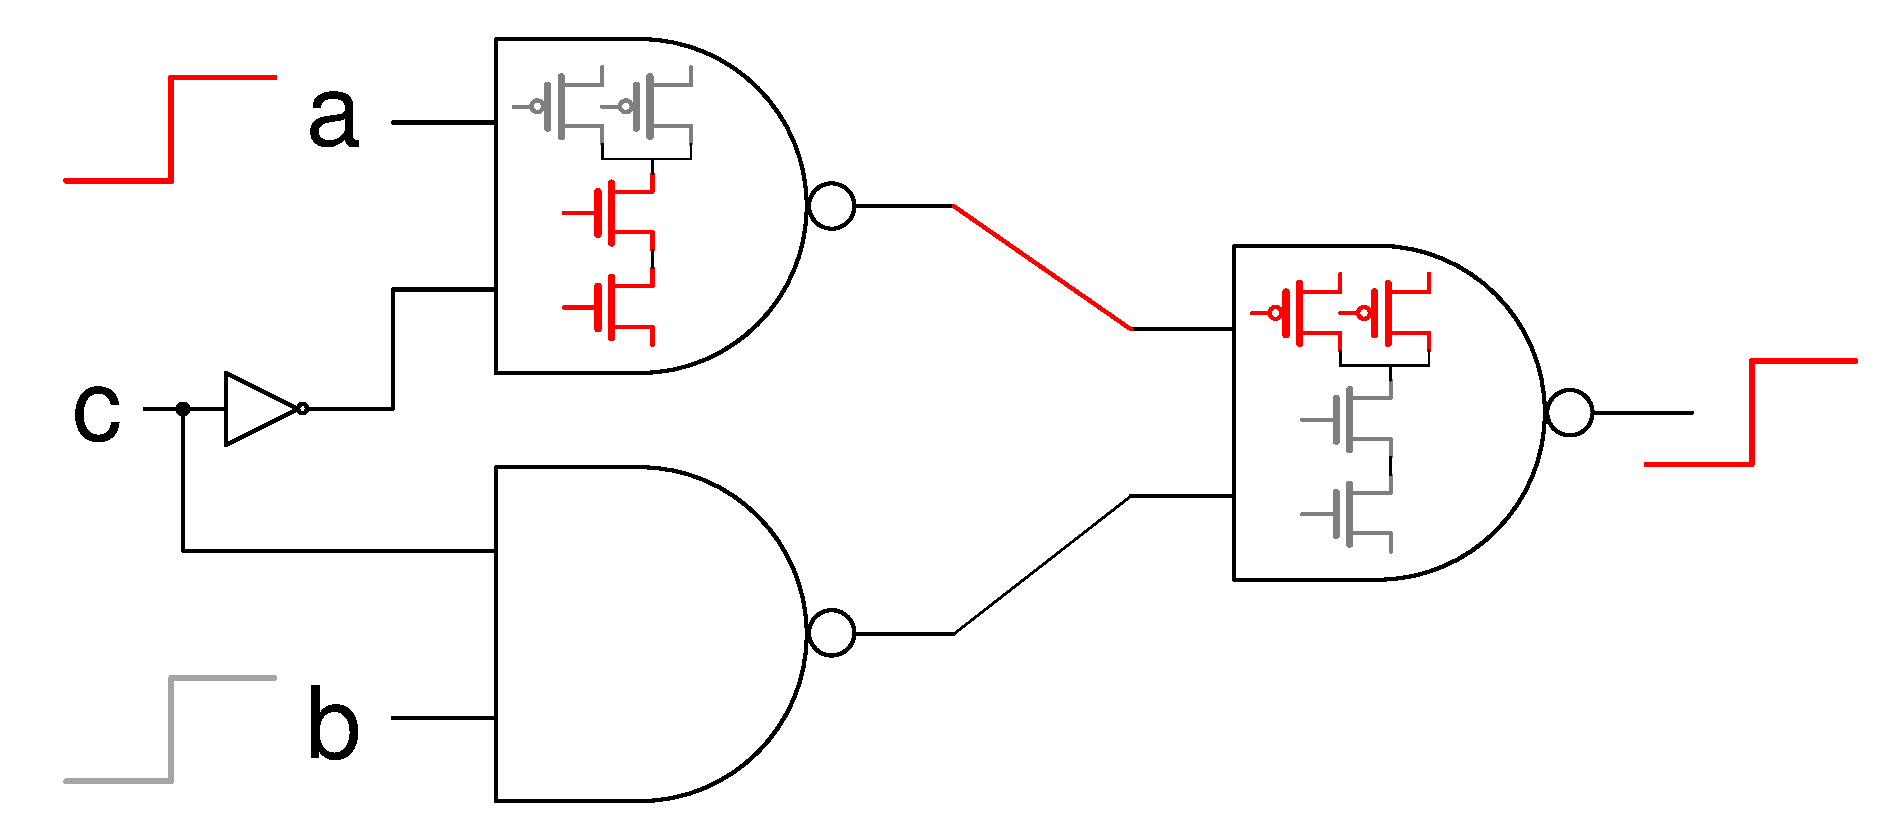
\includegraphics[width=.6\linewidth]{mux_logic_level}
\caption{交换器MUX设计电路图}
\label{fig:mux_logic}
\end{figure}

如图\ref{fig:papuf}所示,修改仲裁型 PUF 的输出,使最后一级交换器输出接入两个触发器 DFF1, DFF2,其中 DFF1 是正边沿锁存, DFF2 是负边沿锁存。复位之后,输入给入一个宽w的脉冲信号,其中上升沿会被 DFF1 采样,$ R_1=sgn(P'D_1 ) $,下降沿则被 DFF2 采样,$ R_2=sgn(P'D_2 ) $ 。输出 $ R=R_1\oplus R_2 $,由于参数 D1 与 D2 独立,所以输出响应R在$ n^2 $维度线性可分,与2个仲裁型 PUF 异或相当,但是面积减小了一半。

\begin{figure}[htb]
\centering
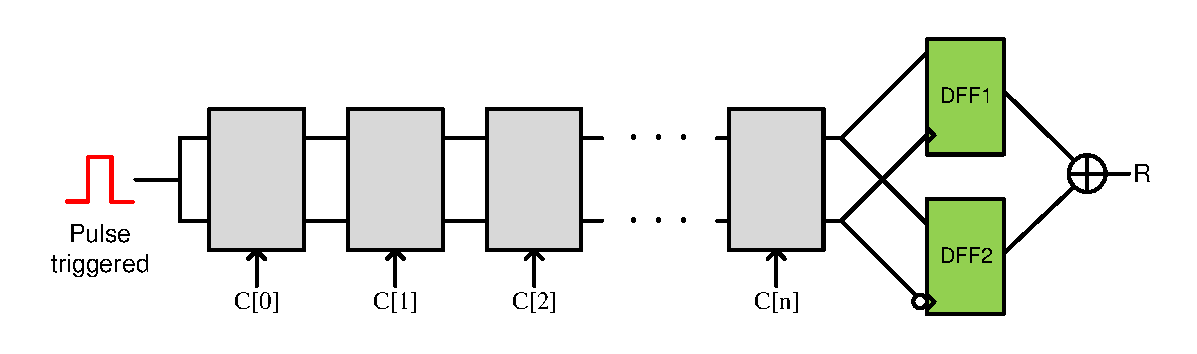
\includegraphics[width=\linewidth]{papuf}
\caption{PAPUF结构图}
\label{fig:papuf}
\end{figure}

下面考虑脉冲宽度w。在经过每一级交换器后,由于延迟时间的不等,w会发生变化,记 $ w_0 (n),w_1 (n) $ 为第n级交换器输出后顶/底两个节点的信号脉宽。
若w足够长,则能都正常通过N级交换器最后被触发器采样;倘若w足够小,那么当经过第i级交换器时,若上升沿延迟远远长于下降沿延迟,则 $ w(i+1)<0 $ (省略掉下标因为具体是哪个节点并不重要)。
这意味着第i级交换器并不会输出脉冲,将这种现象称为短脉冲的``消失''。
为了进一步增加抵抗建模攻击的能力,需要增加模型复杂度。
利用脉冲``消失''属性,令w恰好满足对所有激励有一定概率使得脉冲信号不会传递至寄存器,即在中途``消失''了。
对于消失的脉冲,两个寄存器都会采样出逻辑``0''(或者没有时钟信号,保持原值0)。

\begin{figure}[htb]
\centering
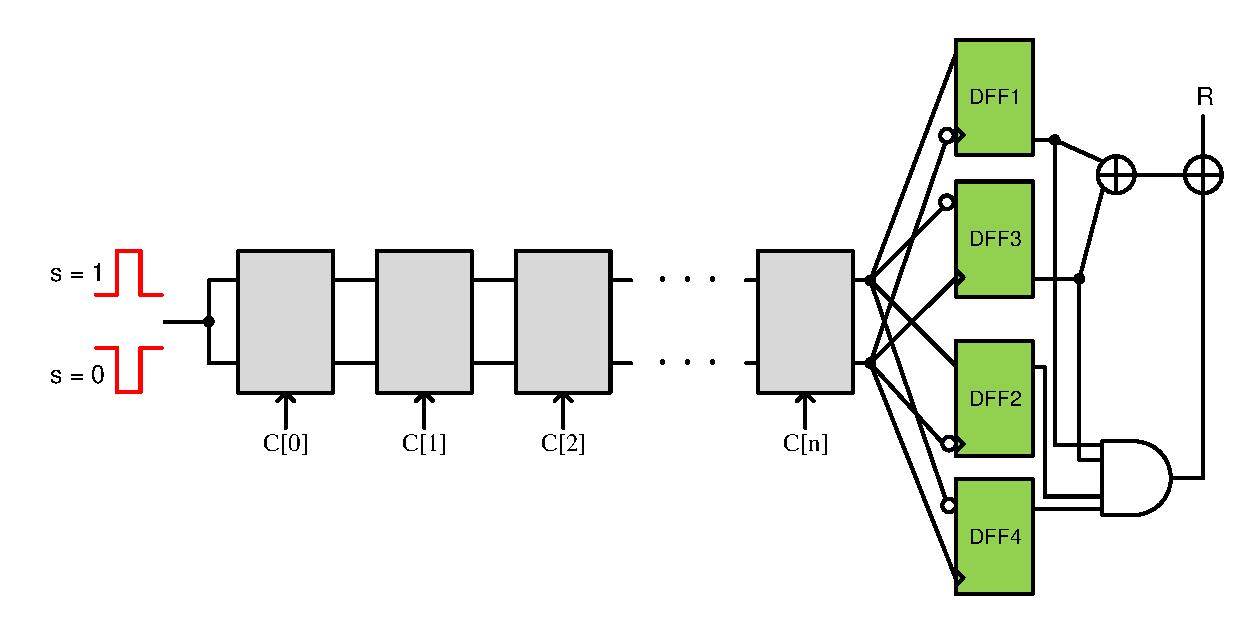
\includegraphics[width=\linewidth]{rpapuf}
\caption{改进的PAPUF结构图}
\label{fig:rpapuf}
\end{figure}

构建如图\ref{fig:rpapuf}所示的电路,输出由4个寄存器DFF1--DFF4组成,分别以正、负边沿采样两个节点。
复位时,先生成随机码s,若s为0,则寄存器复位为0,输入正脉冲$ {p}_0 $;若s为1,则寄存器复位为1,输入负脉冲$ {p}_1 $。
若脉冲信号正常传输至寄存器DFF1--DFF4,则 $ Q_1=r_1,~Q_2=\overline{r_1},~Q_3=r_2,~Q_4=\overline{r_2} $; 若脉冲信号消失,则有 $ Q_1=Q_2=Q_3=Q_4=s $。
输入采用 如下所述的策略:以50\%概率产生一个正脉冲,有50\%概率产生一个负脉冲, $ \mathrm{P}(p_0)=\mathrm{P}(p_1)=0.5  $。
这样,当脉冲正常传输时, DFF1--DFF4 寄存器采样到的值与正负脉冲无关,而当脉冲在中途消失时,则有以下几种情况:

\begin{itemize}
\item 正负脉冲均不能传递过去,则对于正脉冲,$ Q1=Q2=Q3=Q4=0 $;对于负脉冲$ Q1=Q2=Q3=Q4=1 $;
\item 正脉冲可以传递,负脉冲消失。则当s=1时,响应恒为1;
\item 负脉冲可以传递,正脉冲消失。则当s=0时,响应恒为0.
\end{itemize}
考虑整体情况,对于任意激励 $ C_i $,由于正负脉冲发生的概率定为50\%,所以总体响应理论分布仍然是50\%。真值表见表\ref{tab:true-table-rpa}。

\begin{table}[h!]
\centering
\caption{RPAPUF真值表}
\label{tab:true-table-rpa}
\begin{tabular}{c|cccc|c}
\hline
s & $ Q_1 $ & $ Q_2 $ & $ Q_3 $ & $ Q_4 $ & 备注 \\
\hline
x & 0 & 1 & 0 & 1 & 正常传递\\
x & 0 & 1 & 1 & 0 & 正常传递\\
x & 1 & 0 & 0 & 1 & 正常传递\\
x & 1 & 0 & 1 & 0 & 正常传递\\
1 & 1 & 1 & 1 & 1 & 负脉冲消失\\
0 & 0 & 0 & 0 & 0 & 正脉冲消失\\
\hline
\end{tabular}
\end{table}

与普通PUF不同,在具体求值时,需要重复激励K次,若K次结果恒定(或在考虑到噪声情况下大概率为某恒定值),则取本次 CRP;
反之,若K次结果为随机值,则抛弃此激励,取另一激励重复以上步骤。
那么对于 PUF 的使用者来说,代价是 CRP 空间减小了,且求值时间增加了K倍。
而对于攻击者来说,则不能用 XOR PUF 的模型来统一描述所有情况,且取等量训练集 CRP 耗费的时间增加为K倍。

\section{统计分析}\label{sec:rpa_stat}
PAPUF 的模型和统计分布与 XOR PUF 相同,具体参见\ref{sec:relatedwork}节相关内容。
对于改进后 PAPUF(随机 PAPUF,记为 RPAPUF )分析,设在所有 CRP 中,正脉冲消失的概率为$ p_p $,负脉冲消失的概率为$ p_n $, CRP 的总数是 $ M=2^N $。且:

\begin{equation}
R=Q_1\oplus Q_3\oplus (Q_1\cdot Q_2\cdot Q_3\cdot Q_4)
\end{equation}

假设一种理想模型,即在 PAPUF 的 CRP 中``1''严格地占50\%;而在 RPAPUF 中,随机码 s 严格遵循均匀分布。
则在 RPAPUF 中将整个 CRP 集合分为3个子集,记作 $ P_{0}, P_{1}, P_{2} $ ,分别表示脉冲信号都完整传递的 CRP 集合、有且仅有一种脉冲信号完整传递的 CRP 集合和两种脉冲信号全都消失的 CRP 集合。
对于 $ P_0 $, 有响应 $ R(i) = f_{xor}(C_i) $, $ f_{xor} $ 即 XOR PUF 的表征模型,具体参见\ref{subsec:xormethod}节的内容。
而对于 $ P_2 $, 有 $ R(i) = s $。
最后对于 $ P_1 $,若负脉冲没有传递到寄存器,则 $ R(i)= f_{xor}(C_i)+s $ ; 若正脉冲没有传递到寄存器,则 $ R(i)=f_{xor}(C_i)\cdot s $ 。
根据前面的假设,$ P_0 $ 在全集应占比 $ (1-p_p)(1-p_n) $ , $ P(P_1)=p_p+p_n-2p_pp_n $, $ P(P_2)=p_pp_n $。

假设攻击者没有经过多次采样而直接用 XOR PUF 模型进行预测,则在训练集CRP中存在若干``随机点''。
易知,若随机点过少,则不会对建模造成影响,因为SVM学习过程中有``惩罚系数''可以过滤掉这部分数据,但是当随机点在训练CRP中占比上升,则训练效果会直线下降。
图\ref{fig:xor-svm-random}显示了用10000个CRP作为训练集学习 XOR PUF 模型参数,当随机点占比变化时预测率的变化。

\begin{figure}[htb!]
\centering
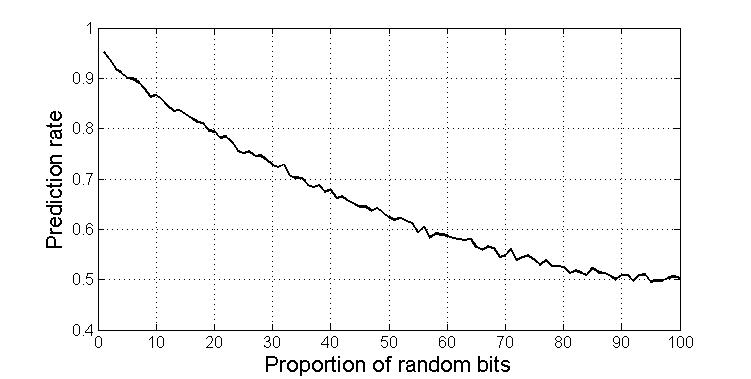
\includegraphics[width=.8\linewidth]{xorpuf_svm_randompoints}
\caption{XOR PUF预测率与训练集随机点占比的关系}
\label{fig:xor-svm-random}
\end{figure}

下面考虑对 RPAPUF 的建模攻击。
首先,攻击者必须对每一个激励重复若干次,以抛弃掉脉冲``消失''的(或``随机''的) CRP,因为消失的响应不满足 XOR PUF 模型;其次,对于剩下的 CRP ,有一部分属于 $ P_1 $ 。 即虽然该部分 CRP 某些脉冲激励``消失''了,但响应输出与随机码 s 无关,因此无法被攻击者过滤掉,所以攻击者只有50\%的概率判断此 CRP 的脉冲是否消失。
对于正常情况,响应仍满足 XOR PUF 的模型,但对于消失脉冲,第i级以后的的交换器不再产生作用,因此攻击者需要遍历N个节点,以寻找在哪个节点脉冲消失了。故建模的复杂度远远超过 $ m\cdot n^2 $ 量级\footnote{$ m $是SVM训练集中CRP个数,$ n^2 $是最小线性可分维度。}。

综上,使用者以 CRP 缩小的代价换取复杂度的显著提升,图\ref{fig:xor-svm-random}显示,为了达到最大效果, 应调节脉宽宽度使得 CRP 全集中至少50\%的脉冲不能传递到寄存器。
故 RPAPUF 以多次求值和 CRP 缩小一半的单价提升了建模复杂度。


\section{仿真验证}\label{sec:rpa_simu}
与\ref{chap:buildingmodel},\ref{chap:dbrpuf}章相同,采用 HSPICE 与 Matlab 结合的方式仿真。
不过由于本结构 RPAPUF 建模困难,采用迭代算法算出每一级交换器的输出延时,并判断该节点脉冲信号是否消失——若消失,则退出迭代,输出寄存器赋值``0''或``1'';否则迭代到N并计算延迟差。

脉冲宽度会显著影响结果,我们取宽度 $ w/d={1,10,100,1000} $,即倍率指数增长,1倍意味着根本没有任何脉冲信号能传递到寄存器,采样的值永远随着脉冲变化,因此响应因为随机值;1000倍意味着所有脉冲都能传递到寄存器,与正负脉冲无关,所以退化到PA PUF 。根据不同的脉宽,统计100个 PUF,每个 PUF 随机输入4096个32位激励得到的响应。图\ref{fig:rpa-single-rand}展示了 RPAPUF 的单次采样下随机性分布示意图。

\begin{figure}[htb!]
\centering
\subfloat[W/D = 1]{
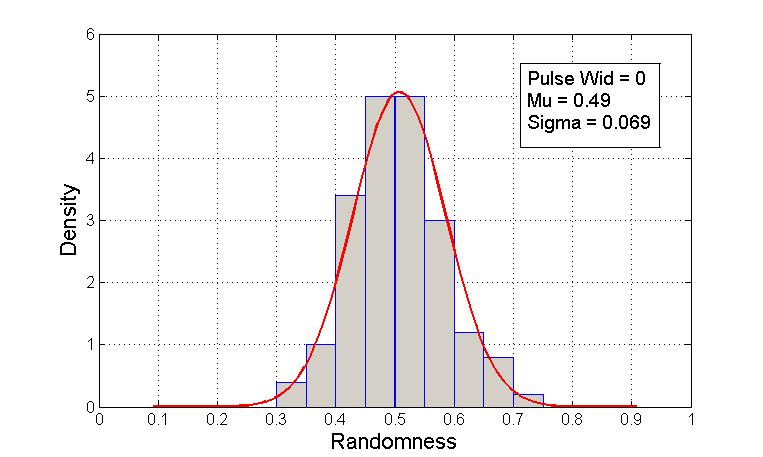
\includegraphics[width=.5\linewidth]{rpapuf_rand_pw0}
}
\subfloat[W/D = 10]{
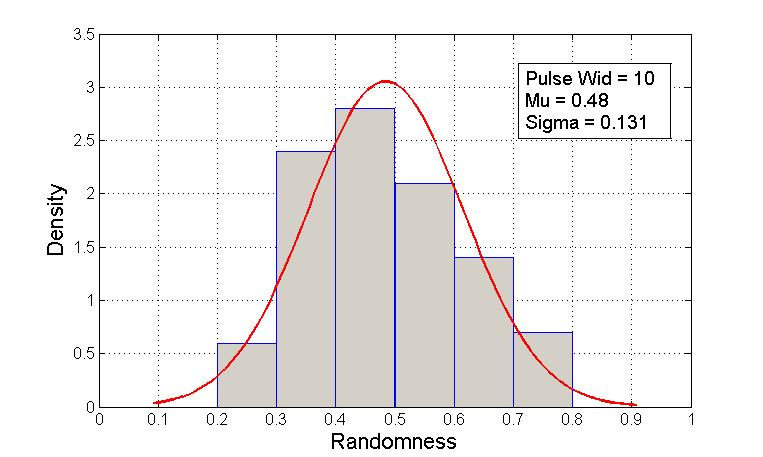
\includegraphics[width=.5\linewidth]{rpapuf_rand_pw10}
}\\
\subfloat[W/D = 100]{
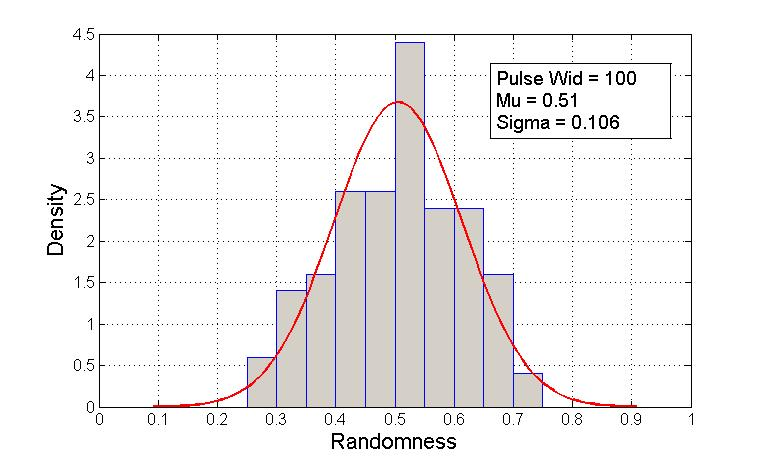
\includegraphics[width=.5\linewidth]{rpapuf_rand_pw100}
}
\subfloat[W/D = 1000]{
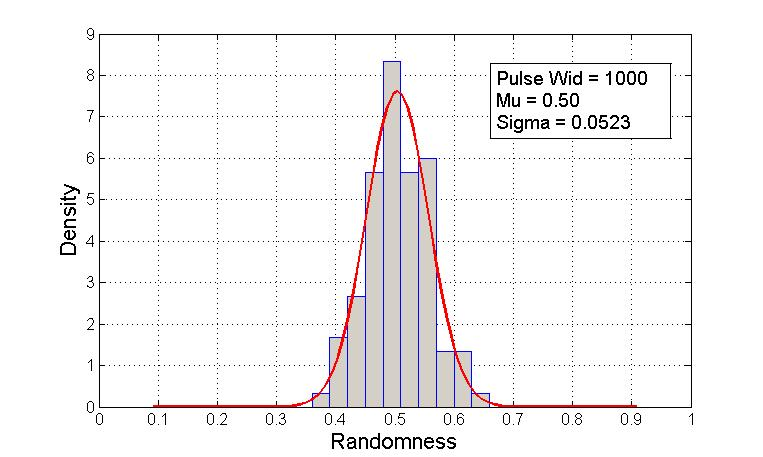
\includegraphics[width=.5\linewidth]{rpapuf_rand_pw1000}
}
\caption{RPAPUF单次采样随机性分布柱状图}
\label{fig:rpa-single-rand}
\end{figure}

可以看出,随着w的变化,R的输出分布变化并不明显,说明宏观上难以分辨出脉冲信号是否传递到寄存器,若采用 XOR PUF 建模方法,则会严重受到随机脉冲的干扰。
图\ref{fig:rpa-k100-rand}是脉宽延时比设为100时经过100次采样过滤后的随机性分布。

\begin{figure}[htb!]
\centering
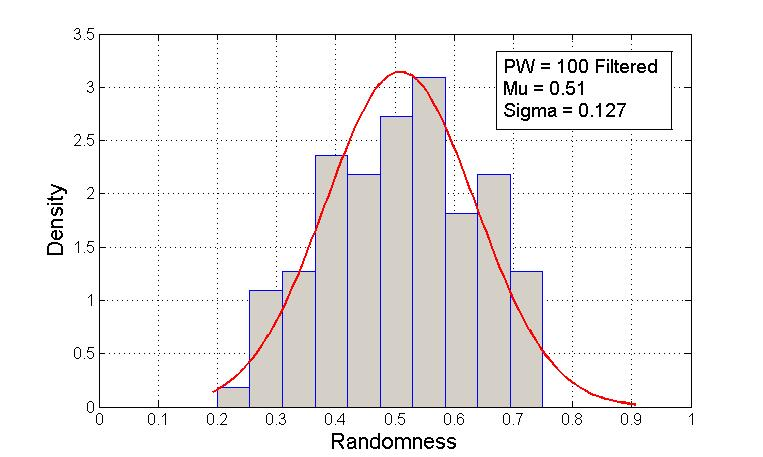
\includegraphics[width=.8\linewidth]{rpapuf_rand_pw100_filter}
\caption{RPAPUF 100次采样过滤随机响应后的随机性分布}
\label{fig:rpa-k100-rand}
\end{figure}

我们尝试用 XOR PUF 的模型对 RPAPUF 进行建模攻击, 图\ref{fig:rpa-svm}展示了对 32 位 RPAPUF 的攻击结果,虚线为训练集 CRP 单次采样的结果,即不分辨``消失''脉冲;
实线为训练集 CRP 多次采样,抛弃随机变化的点,能够过滤到部分``消失''脉冲。
图\ref{fig:rpa-svm-devices}显示训练集CRP在10000个的情况下,不同PUF在SVM建模后的预测率,横轴对应的是不同的器件。
可以看出无论响应过滤与否均不能达到很好的效果, 即使过滤掉部分随机 CRP,预测率并不会随着训练集 CRP 增加而增多。
同时也看出,随着片间分布变化,在某些情况下,恰好随机脉冲作用不明显(比如几乎没有消失,或者消失掉的部分恰好符合模型函数),使得有几个 PUF器件的点预测率非常高,这给我们留下了下一步的工作——分析随机脉冲在片内和片间的分布,尤其是脉冲宽度与工艺之间取何值最优。在现在的工作中囿于计算能力,不能再进一步分析。

\begin{figure}[htb!]
\centering
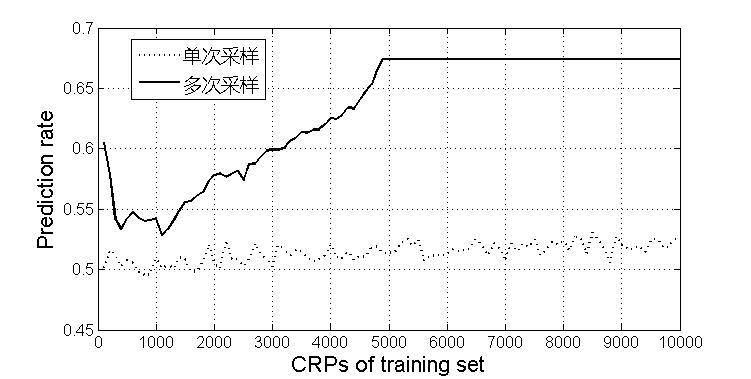
\includegraphics[width=.8\linewidth]{rpa_svm_single}
\caption{RPAPUF SVM预测结果(单一器件)}
\label{fig:rpa-svm}
\end{figure}

\begin{figure}[htb!]
\centering
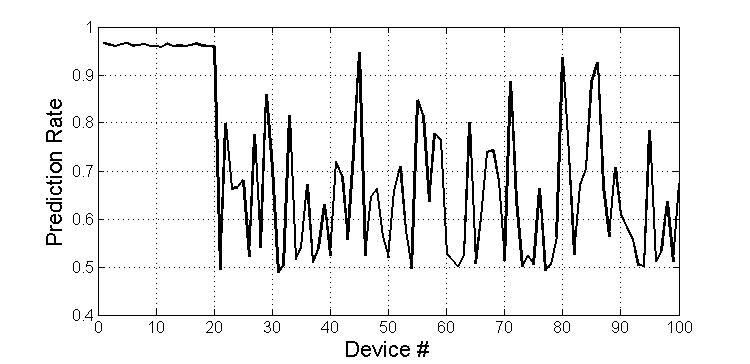
\includegraphics[width=.8\linewidth]{rpa_svm_devices}
\caption{RPAPUF SVM预测结果(跨器件统计)}
\label{fig:rpa-svm-devices}
\end{figure}

\section{几种PUF结构横向对比暨本章小结}\label{sec:rpa_summary}
本节提出并分析了新型随机脉冲型 PUF。
至此,本文一共分析了5种不同的 PUF 结构,表\ref{tab:puf_cmp}对其基本信息做了整理,表\ref{tab:puf_nist}展示了所有 PUF 的 NIST 测试结果\footnote{每PUF测试100个器件仿真,收集32768比特响应。Random 测试由于数据不支持没有结果。}。
在图\ref{fig:pufs_rand}中绘出所有 PUF 的随机性分布拟合曲线,图\ref{fig:pufs_uniq}则绘出了独特性的拟合曲线。

\begin{table}[htb]
\centering
\caption{PUF特征对比}\label{tab:puf_cmp}
\begin{tabular}{cccc}
\hline
PUF			& CRP空间	   & 最小线性可分空间维度 & 面积开销\\
\hline
Arbiter PUF & $ 2^N $ 	& N & N个交换器 			\\
2-XOR PUF	& $ 2^N $ 	& $ N^2 $ & 2N个交换器	    \\
BRPUF		& $ 2^N $ 	& N & 2N个与非门和多路器 	 \\
4-DBRPUF	& $ 2^N $ 	& N & N+4个交换器和8个与非门 \\
RPAPUF		& $ 2^{N-1} $ & - & N个交换器 		   \\
\hline
\end{tabular}
\end{table}

\begin{table}[htb]
\centering
\caption{PUF NIST测试通过率}
\label{tab:puf_nist}
\begin{tabular}{cccccc}
\hline
NIST Test & Arbiter & 2-XOR & BRPUF & 4-DBRPUF & RPAPUF \\
\hline
Frequency & 7 & 15 & 2 & 8 & 7\\
Block Frequency & 29 & 25 & 5 & 20 & 29\\
Cumulative Sums & 7 & 15 & 2 & 7.5 & 7.5\\
Runs & 12 & 17 & 5 & 11 & 13 \\
Longest Run & 33 & 27 & 4 & 20 & 29 \\
Rank & 99 & 100 & 71 & 99 & 100\\
FFT & 84 & 78 & 17 & 50 & 83 \\
Universal & 0 & 0 & 0 & 0 & 0 \\
Approximate Entropy & 39 & 32 & 4 & 19 & 37\\
Serial & 87.5 & 83.5 & 22.5 & 58 & 86.5\\
Linear Complexity & 100 & 98 & 90 & 98 &99 \\
Random Excursions & - & - & - & - & -\\
Random Excursions Variant & - & - & - & - & -\\
Overlapping Template & 61 & 55 & 10 & 28 & 53 \\
Nonperiodic Template & 88.4 & 86.4 & 34.0 & 70.1 & 88.3\\
\hline
\end{tabular}
\end{table}

\begin{figure}[htb]
\centering
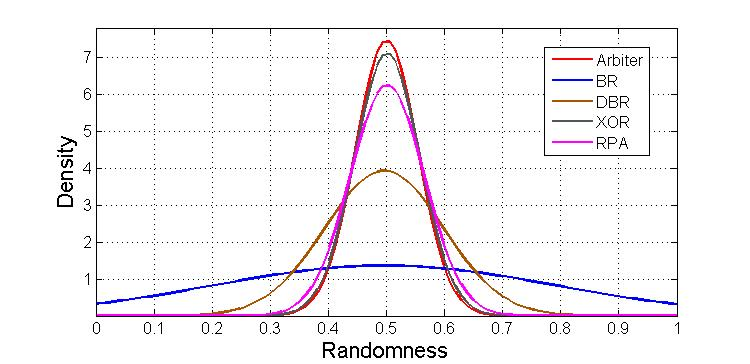
\includegraphics[width=.8\linewidth]{rand_5pufs}
\caption{PUF随机性分布拟合曲线}
\label{fig:pufs_rand}
\end{figure}

\begin{figure}[htb]
\centering
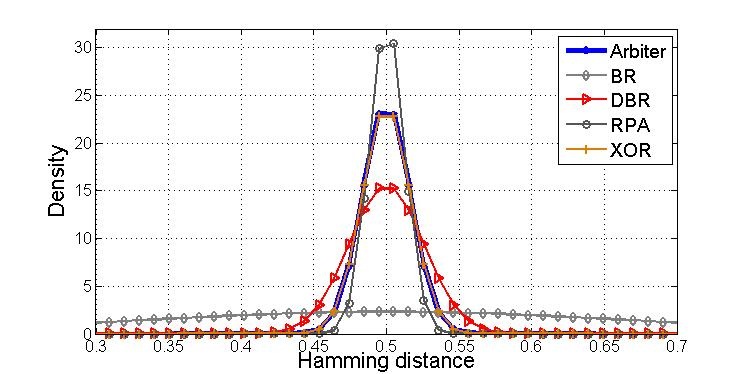
\includegraphics[width=.8\linewidth]{uniq_5pufs}
\caption{PUF独特性分布拟合曲线}
\label{fig:pufs_uniq}
\end{figure}

可以看出,综合比较, DBRPUF 优于 BRPUF,但两者相比于传统仲裁型 PUF 在随机性上仍不足。改进后的 XOR PUF 和 RPAPUF 则在统计结果上优于传统仲裁型 PUF,而本文所提出的 RPAPUF 在面积上优于 XOR PUF。最后,图\ref{fig:svm_all}给出了 SVM 机器学习结果,根据我们的建模,仲裁型 PUF 和 BRPUF 能够用1000个训练集达到95\%以上的预测成功率,而 XOR PUF 则需要超过5000个训练集,耗费数倍时间才能达到95\%的成功率。对于 RPAPUF,因为建模困难,我们用 XOR PUF 的模型进行学习,可以看出直接学习的成功率仅有50\%,根随机猜测一样,而经过多次采样过滤后的预测成功率最高也仅达到67\%,在有限的时间内并不能更进一步提升其预测率,故安全性上评价总结见表\ref{tab:puf_cmp}。

\begin{figure}[htb!]
\centering
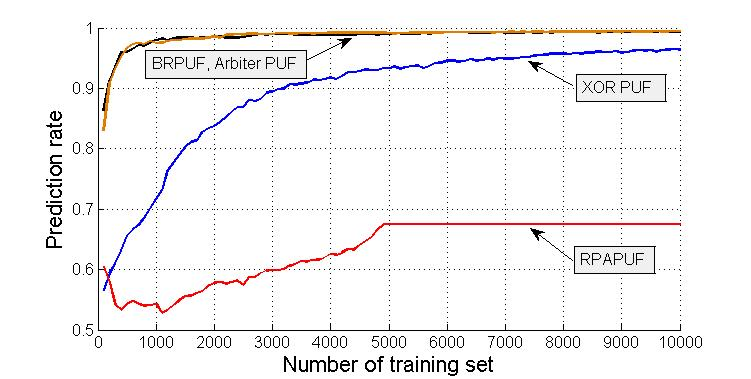
\includegraphics[width=.8\linewidth]{svm_all}
\caption{不同PUF SVM预测率对比}
\label{fig:svm_all}
\end{figure}

	% 结论。
	% vim:ts=4:sw=4
% Copyright (c) 2014 Casper Ti. Vector
% Public domain.

\specialchap{结论}\label{chap:conclusion}
\section{全文总结}
在密码学研究中,单向函数是构造高层次密码协议的基础。 PUF 作为物理不可克隆函数,是基于人类不可知的物理原理构造的单向函数,在密码学领域有着重要应用。

本文从数学原理出发,用统计方法和机器学习建模攻击对仲裁型 PUF、异或 PUF、双稳态环路 PUF 进行分析。
通过模型公式对 Strong PUF 的安全性原理进行了总结,分析并指出了异或结构的安全性原理,和双稳态环路 PUF 的统计性失准的原因:因为 BRPUF 在求值过程中累积了所有逻辑门的延迟偏差,导致结果的统计方差大大增加。
根据建模分析,在模型线性表达式或近似线性表达式中,最小线性可分维度的大小决定了机器学习的拟合时间代价。

为了提升 PUF 的安全性,本文提出了两种新型 PUF 结构,其中第\ref{chap:dbrpuf}章的 DBRPUF 针对 BRPUF 进行改进,消除了延迟偏差累积,因此改善了统计测试结果,但相比传统异或结构仍显不足;
第\ref{chap:rpapuf}章新提出的随机脉冲信号的 RPAPUF,利用逻辑门的双边延迟构造出复杂的结构,随机选择脉冲输入,利用脉冲传递路程长短``欺骗''攻击者,使其不能分辨出哪些响应符合模型计算结果,哪些是随机项,从而使建立模型需要花费极大开销,相对传统结构大大加强了 PUF 对于建模攻击的抵御能力。

在实验上,为了缩短仿真时间,本文利用 HSPICE 和 Matlab 结合的方法,HSPICE 负责仿真基本逻辑门的工艺波动,Matlab 负责建立由多个逻辑门组成的电路结构,并通过简化模型静态仿真电路行为,使得多比特 PUF 可以在有限时间内仿真完成。
因此本文验证了所有 PUF 结构,并在 Altera FPGA 上实现并比较了 Arbiter PUF,BRPUF 和 DBRPUF 结构。结果证实了理论分析,证明了本文提出结构的可行性。

最后,本文研究仍存在一些不足之处。
首先,本文采用的统计分析基于工艺波动服从正态分布这一假设,但是在不同工艺,尤其是深亚微米制程下,这一假设不一定满足,因此不同工艺对于 PUF 的输出影响需要进一步的实验验证。
其次,FPGA 的实现存在布线偏差,且实验用 FPGA 数量不足,不能很好的反应不同 PUF 之间的片间分布差异,因此更精确的验证应该采用全定制方法设计 PUF。
最后,本文尚没有对 PUF 的稳定性进行验证,包括电压波动稳定性、环境温度波动稳定性、和时间稳定性。

我们希望在后续的研究中将提出的 RPAPUF 应用于高层次密码协议,从而分析 PUF 的实用性开销和代价,并通过流片进一步验证新型 PUF 结构在不同工艺下的表现,以及在不同电源电压和环境温度下稳定性表现。


\section{前景展望}

PUF 的安全性始终是 PUF 的终极评价标准,而 PUF 的安全性设计和针对这项设计的攻击一直以来都是彼此的博弈。
目前,侵入式探查、旁道攻击等崭新方式给 PUF 带来更多的设计挑战,而全新的工艺技术和期间技术又给 PUF 设计带来了新的可能\supercite{delvaux2013side,merli2013localized,helfmeier2013cloning}。
不仅有双值逻辑的数字电路 PUF,还有基于 RRAM、模拟电路实现的 PUF 具有更高的非线性特点\supercite{liu2015experimental,chen2015utilizing}。
这些都使得未来的研究非常有趣,无论攻防哪一方占得先机,都会给这一领域的研究带来新的启迪和方向。

再者,安全应用的最终实现还是种种密码协议。
基于 PUF 的密码协议越来越多的涌现出来,比如有基础协议``不经意传输协议''的 PUF 实现\supercite{ruhrmair2010oblivious}, FPGA 上的 IP 保护\supercite{kumar2008butterfly}, ``比特承诺协议''\supercite{ruhrmair2013practical}等等。
尽管 PUF 有着天然的安全属性,但是协议的复杂性使基于 PUF 的协议构建非常困难,尤其是每一篇新的协议模型总会伴随而来一篇攻击方法\supercite{ruhrmair2013pufs}。
在未来,相信随着 PUF 研究的深入,能够找到一种完美利用 PUF 特点,真正实现高效、低功耗、不可克隆的密码协议,使得 PUF 应用于千千万万移动端安全芯片,真正为千家万户的安全护航。

	% 正文中的附录部分。
%	\appendix
	% 排版参考文献列表。
	\printbibliography[
		% 使“参考文献”出现在目录中;如果同时要使参考文献列表参与章节编号,
		% 可将“bibintoc”改为“bibnumbered”。
		heading = bibintoc,
		% 单独设定排序方案。此设定会局部覆盖之前的全局设置。
		% 注:只有同时使用 2.x 或之后版本的 biblatex 和相应兼容版本的 biber,
		% 才能对每个 \printbibliography 命令采用不同的排序方案,
		% 否则只能在载入 biblatex 宏包时就(全局)指定排序方案。
		% 在这样的情况下,请去掉所有的 sorting 选项,否则可能出错。
		% 此外,biblatex 3.0 中 \printbibliography 的 sorting 选项失效,
		% 详见 biblatex-caspervector 的文档。
		sorting = none
	]
	% 各附录。
%	% vim:ts=4:sw=4
% Copyright (c) 2014 Casper Ti. Vector
% Public domain.

\chapter{附件}
% 中文测试文字。




	% 以下为正文之后的部分,默认不进行章节编号。
	\backmatter
	% 发表文章
	% vim:ts=4:sw=4
% Copyright (c) 2014 Casper Ti. Vector
% Public domain.

\specialchap{攻读硕士学位期间发表的论文和申请的专利}
\noindent
[1] \textbf{\underline{Wenyi Tang}}, Song Jia, and Yuan Wang, \textit{``A Dual-voltage Single-rail Dynamic {DPA}-resistant Logic Based on Charge Sharing Mechanism''}, Electron Devices and Solid-State Circuits (EDSSC), 2015 IEEE International Conference on, \textbf{2013}: 483-486

\noindent
[2] \textbf{\underline{Wenyi Tang}}, Song Jia, and Yuan Wang, \textit{``A Short-time Three-phase Single-rail Precharge Logic Against Differential Power Analysis''}, IEICE Transactions on Electronics (Accepted)

	% 致谢。
	% vim:ts=4:sw=4
% Copyright (c) 2014 Casper Ti. Vector
% Public domain.

\chapter{致谢}
% 中文测试文字。



	% 原创性声明和使用授权说明。
	% vim:ts=4:sw=4
%
% Copyright (c) 2008-2009 solvethis
% Copyright (c) 2010-2015 Casper Ti. Vector
% All rights reserved.
%
% Redistribution and use in source and binary forms, with or without
% modification, are permitted provided that the following conditions are
% met:
%
% * Redistributions of source code must retain the above copyright notice,
%   this list of conditions and the following disclaimer.
% * Redistributions in binary form must reproduce the above copyright
%   notice, this list of conditions and the following disclaimer in the
%   documentation and/or other materials provided with the distribution.
% * Neither the name of Peking University nor the names of its contributors
%   may be used to endorse or promote products derived from this software
%   without specific prior written permission.
%
% THIS SOFTWARE IS PROVIDED BY THE COPYRIGHT HOLDERS AND CONTRIBUTORS "AS
% IS" AND ANY EXPRESS OR IMPLIED WARRANTIES, INCLUDING, BUT NOT LIMITED TO,
% THE IMPLIED WARRANTIES OF MERCHANTABILITY AND FITNESS FOR A PARTICULAR
% PURPOSE ARE DISCLAIMED. IN NO EVENT SHALL THE COPYRIGHT HOLDER OR
% CONTRIBUTORS BE LIABLE FOR ANY DIRECT, INDIRECT, INCIDENTAL, SPECIAL,
% EXEMPLARY, OR CONSEQUENTIAL DAMAGES (INCLUDING, BUT NOT LIMITED TO,
% PROCUREMENT OF SUBSTITUTE GOODS OR SERVICES; LOSS OF USE, DATA, OR
% PROFITS; OR BUSINESS INTERRUPTION) HOWEVER CAUSED AND ON ANY THEORY OF
% LIABILITY, WHETHER IN CONTRACT, STRICT LIABILITY, OR TORT (INCLUDING
% NEGLIGENCE OR OTHERWISE) ARISING IN ANY WAY OUT OF THE USE OF THIS
% SOFTWARE, EVEN IF ADVISED OF THE POSSIBILITY OF SUCH DAMAGE.

{
	\CTEXsetup[
		format+ = {\centering}, beforeskip = {40bp}, afterskip = {15bp}
	]{section}

	\specialchap{北京大学学位论文原创性声明和使用授权说明}
	\mbox{}\vspace*{-3em}
	\section*{原创性声明}

	本人郑重声明:
	所呈交的学位论文,是本人在导师的指导下,独立进行研究工作所取得的成果。
	除文中已经注明引用的内容外,
	本论文不含任何其他个人或集体已经发表或撰写过的作品或成果。
	对本文的研究做出重要贡献的个人和集体,均已在文中以明确方式标明。
	本声明的法律结果由本人承担。
	\vskip 1em
	\rightline{%
		论文作者签名:\hspace{5em}%
		日期:\hspace{2em}年\hspace{2em}月\hspace{2em}日%
	}

	\section*{%
		学位论文使用授权说明\\[-0.33em]
		\textmd{\zihao{5}(必须装订在提交学校图书馆的印刷本)}%
	}

	本人完全了解北京大学关于收集、保存、使用学位论文的规定,即:
	\begin{itemize}
		\item 按照学校要求提交学位论文的印刷本和电子版本;
		\item 学校有权保存学位论文的印刷本和电子版,
			并提供目录检索与阅览服务,在校园网上提供服务;
		\item 学校可以采用影印、缩印、数字化或其它复制手段保存论文;
		\item 因某种特殊原因需要延迟发布学位论文电子版,
			授权学校在 $\Box$\nobreakspace{}一年 /
			$\Box$\nobreakspace{}两年 /
			$\Box$\nobreakspace{}三年以后在校园网上全文发布。
	\end{itemize}
	\centerline{(保密论文在解密后遵守此规定)}
	\vskip 1em
	\rightline{%
		论文作者签名:\hspace{5em}导师签名:\hspace{5em}%
		日期:\hspace{2em}年\hspace{2em}月\hspace{2em}日%
	}

	% 若需排版二维码,请将二维码图片重命名为“barcode”,
	% 转为合适的图片格式,并放在当前目录下,然后去掉下面 2 行的注释。
	%\vfill\noindent
	%\includegraphics[height = 5em]{barcode}
}


\end{document}

